\documentclass[11pt,a4paper]{article}

% Page geometry
\usepackage[top=2.5cm, bottom=2.5cm, left=2.5cm, right=2.5cm]{geometry}

% Typography and encoding
\usepackage[T1]{fontenc}
\usepackage[utf8]{inputenc}
\usepackage{lmodern}
\usepackage{microtype}

% Mathematics
\usepackage{amsmath,amssymb,amsthm}

% Tables and arrays
\usepackage{booktabs}
\usepackage{tabularx}
\usepackage{array}
\usepackage{makecell}
\usepackage{multirow}

% Graphics and floats
\usepackage{graphicx}
\usepackage{float}
\usepackage{placeins}

% Utility packages
\usepackage{cite}
\usepackage{seqsplit}
\usepackage{url}
\usepackage{xcolor}
\usepackage{authblk}

% Additional formatting packages
\usepackage{caption}
\captionsetup[figure]{labelfont=bf,labelsep=space}
\captionsetup[table]{labelfont=bf,labelsep=space}
\usepackage{adjustbox}

% Hyperlinks
\usepackage[colorlinks=true,linkcolor=blue!75!black,citecolor=blue!75!black,urlcolor=blue!75!black]{hyperref}

% Theorem environments
\theoremstyle{plain}
\newtheorem{theorem}{Theorem}
\newtheorem{proposition}{Proposition}
\newtheorem{lemma}[proposition]{Lemma}
\newtheorem{corollary}[proposition]{Corollary}

\theoremstyle{definition}
\newtheorem{definition}{Definition}
\newtheorem{example}{Example}

\theoremstyle{remark}
\newtheorem{remark}{Remark}

% Supplementary numbering
\renewcommand{\thefigure}{S\arabic{figure}}
\renewcommand{\thetable}{S\arabic{table}}
\renewcommand{\theproposition}{S\arabic{proposition}}
\renewcommand{\thelemma}{S\arabic{lemma}}
\renewcommand{\thecorollary}{S\arabic{corollary}}

% Title and authors
\title{\textbf{Supporting Information: Exact Policy-Aware Regression Diagnosis for Precision-Constrained Threshold Selectors}}

\author[1]{Thien Bao Nguyen\thanks{Corresponding author. Email: \texttt{baont@ueh.edu.vn}}}
\author[1]{Bao Tran Hoang\thanks{Email: \texttt{tranhoang.31251027696@st.ueh.edu.vn}}}
\author[1]{The Dang Khoa Tran\thanks{Email: \texttt{khoatran.31251020280@st.ueh.edu.vn}}}
\author[1]{Bao Han Nguyen\thanks{Email: \texttt{hannguyen.31251027458@st.ueh.edu.vn}}}
\author[1]{Trong Minh Nguyen\thanks{Email: \texttt{minhnguyen.31251023499@st.ueh.edu.vn}}}
\author[1]{Gia Han Tran\thanks{Email: \texttt{hantran.31251027103@st.ueh.edu.vn}}}
% Affiliation
\affil[1]{Institute of Intelligent and Interactive Technologies (3i Institute),
College of Technology and Design (CTD),
University of Economics Ho Chi Minh City (UEH),
Ho Chi Minh City, Vietnam}

\date{\today}

\emergencystretch=3em

\begin{document}

\maketitle

\noindent\textbf{Supporting Information Document} \\
Companion to: \textit{Exact Policy-Aware Regression Diagnosis for Precision-Constrained Threshold Selectors}

\begin{abstract}
This document provides the complete formal diagnostic specifications, proofs, extended empirical validity studies, engineering feasibility benchmarks, algorithmic cost decompositions, reproducibility manifests, and conceptual foundations supporting the main manuscript. All sections S1--S24, Tables S1--S17, Figures S1--S2, and formal results S1--S7 are fully indexed and cross-referenced with the numbered bibliography [1]--[29].
\end{abstract}

\vspace{1em}

\section*{Document Navigation and Reading Guide}\phantomsection\label{sec:nav}
References correspond directly to the main manuscript bibliography. This supplement is organized by evidential role: formal assumptions and proofs come first (Part A), followed by empirical validity (Part B), engineering feasibility (Part C), reproduction protocols and lineage (Part D), and conceptual foundations (Part E). Table and figure numbers follow this reading sequence.

\section*{A Formal diagnostic method and proofs}\phantomsection


\subsection*{S1 Core proof obligations and numerical interface semantics}\phantomsection\label{sec:s1}


\subsubsection*{S1.1 Contract and complete finite partition}\phantomsection\label{sec:s1_1}

Fix N > 0 aligned observations with unique IDs, binary labels and finite old/new scores. Each version has its own finite family of nonempty threshold candidates, indexed by s as in Main Section 2.1. Candidate j has actual positive count k and size n; equal scores enter together. Inclusive feasibility compares the rational policy with k/n, following constrained threshold classification and ranking formulations \cite{rath2022optimizing,mackey2018constrained,tasche2018plugin}. Priority is a fixed total order independent of the policy; for the reference contract it is lexicographic in actual positive count and selected size. No feasible candidate or an all-negative label vector gives the empty selected set. Alternative declared contracts may use different fixed feasibility coefficients; these must be enumerated separately and kept distinct from the actual-positive priority. Policies lie in $\mathcal{A} = [L, H]$, with rational $0 \le L < H \le 1$. These assumptions concern fixed empirical observations, not population precision or arbitrary executable behavior.

\begin{proposition}[Finite Partition]\label{prop:s1}
Let B be {L,H} together with every exact candidate feasibility ratio from both versions strictly inside A. Partition A into the singleton at each element of sorted B and the open intervals between consecutive elements. On any open atom, $\alpha$ cannot cross a feasibility ratio, so every candidate feasibility predicate is constant. Fixed priority and abstention then make the winning membership constant. Thus equality at every singleton and one point of every nonempty open atom is necessary and sufficient for equality on A. Evaluating singletons separately preserves inclusive endpoint ownership; strict feasibility changes their outcome but not the required critical set. A midpoint argument is sound only after deriving the complete B independently.
\end{proposition}

\subsubsection*{S1.2 Prefix membership equality and producer cost}\phantomsection\label{sec:s1_2}

\begin{lemma}[Equal Finite Prefixes]\label{lem:s2}
Let the old and new winners be prefixes of their respective score orders, with sizes n and m and zero-based new ranks r\_new(i). If n $\neq$ m, the sets differ. If n = m = 0, both are empty. Otherwise equality holds exactly when every old selected ID has new rank below n. Necessity follows from equality. For sufficiency this rank condition gives containment in the new prefix, and equal finite cardinality gives equality. Prefix maxima of new ranks in old order answer this condition in constant time after linear preprocessing. A changed-membership ID is a directly checkable witness; a single witness does not enumerate every changed ID.
\end{lemma}
\begin{proposition}[Sweep and Complexity]\label{prop:s3}
As $\alpha$ increases, a candidate that becomes infeasible never becomes feasible again. Start with all candidates in a fixed-priority heap and discard infeasible top candidates until the top is feasible or the heap is empty. Each candidate is inserted once and removed at most once; no monotonicity of empirical precision along the score order is needed. Sorting scores, forming the critical union and sweeping K atoms therefore cost $\mathcal{O}(N \log N + G \log G + K)$ under unit-cost rational arithmetic, where G is the total candidate count and K is the critical-value count up to a constant-factor number of atoms. Retained ranks, candidates and cells require $\mathcal{O}(N + G + K)$ auxiliary storage. Scanning N rows for each of D distinct divergent winner pairs adds $\mathcal{O}(ND)$ witness/count work. Fraction comparison has operand-dependent bit cost; hashing and serialization are additional measured work. A higher-priority feasible candidate cannot be hidden below an infeasible heap top after all infeasible tops are discarded.
\end{proposition}

\subsubsection*{S1.3 Streaming independent consumption}\phantomsection\label{sec:s1_3}

\begin{lemma}[Suffix Winner]\label{lem:s4}
The consumer independently enumerates each actual threshold mask, counts its positives and size, records its exact feasibility ratio and fixed priority, then releases the mask. Sort descriptors by nondecreasing feasibility ratio p. At $\alpha$, inclusive feasibility is precisely the suffix beginning at lower\_bound(p, $\alpha$), while strict feasibility begins at upper\_bound(p, $\alpha$). Reverse induction computes the maximum priority of each suffix: its winner is the better of the current descriptor and the already computed next-suffix winner. The query therefore returns the same winner as exhaustive enumeration. Within a nested candidate family, equal selected size identifies the same prefix, so a priority tie does not hide another membership.
\end{lemma}
\begin{proposition}[Consumer Obligations and Cost]\label{prop:s5}
First validate the input digest, declared contracts, ordered coverage and unique endpoint ownership. Independently derive all critical values and probe them and one midpoint per open atom; additionally check certificate boundaries and their open-cell representatives. Proposition~\ref{prop:s1} and Lemma~\ref{lem:s4} supply the correct winner on every atom. Reconstruct current winner memberships directly from original scores and descriptors; compare actual bitsets, not just counts. Check each cell verdict, witness ID and membership, changed-row count and the independently accumulated divergent length and Boolean equivalence. Acceptance satisfies the finite-domain obligations conditional on these algorithms and their implementations; the claim is not a proof-assistant verification. Only current masks and descriptors are retained, giving $\mathcal{O}(N + G + K + C)$ auxiliary descriptors plus operand storage for C certificate cells. Threshold enumeration and winner reconstruction can still require $\mathcal{O}(NG)$ work; ratio sorting and bisections add $\mathcal{O}(G \log G + (K+C) \log G)$, and probe sorting adds $\mathcal{O}(C \log C + K \log K)$. Split-tie ordering can add $\mathcal{O}(N \log N)$. Quadratic work remains possible when G = N.
\end{proposition}

\subsubsection*{S1.4 Exact binary64 guard cuts}\phantomsection\label{sec:s1_4}

\begin{lemma}[Nearest-Even Guard Preimage]\label{lem:s6}
Under IEEE 754 roundTiesToEven semantics \cite{ieee2019floating}, let p be an actual finite nonnegative binary64 empirical precision returned by the public selector, q its next larger binary64 value, and c their exact rational midpoint. Convert a rational policy $\alpha$ with CPython nearest-even float($\alpha$). Monotonic rounding maps every $\alpha$ below c to a value at most p and every $\alpha$ above c to a value at least q. At c the even significand wins. Consequently the inclusive public guard p $\ge$ float($\alpha$) holds below c, and at c exactly when p is the even neighbor. A public guard therefore has an exact rational cut with explicit closure. Union these cuts with the exact-reference k/n cuts and domain endpoints; Proposition~\ref{prop:s1} applies again because the candidate source, scores, labels and priority are policy independent. Actual public-selector calls at every resulting breakpoint and midpoint check this guard mapping on the recorded runtime. This argument excludes alternative rounding modes, hidden state and additional policy-dependent branches. A rational/binary64 interface differential alone is not a confirmed upstream defect.
\end{lemma}

\subsubsection*{S1.5 PSC and endpoint-only divergence}\phantomsection\label{sec:s1_5}

\begin{corollary}[Length Does Not Establish Equivalence]\label{cor:s7}
Disjoint open atoms have additive exact rational lengths, while singletons have zero Lebesgue measure. PSC is the sum of divergent open-atom lengths divided by H-L. Full equivalence implies PSC = 0, but zero PSC does not imply equivalence. For labels $[1, 0]$, scores $[1, 0]$ and A = $[1/2, 1]$, inclusive and strict feasibility select different memberships at 1/2 and at 1, but agree on the intervening open interval. Their PSC is zero. Certificates must therefore retain the Boolean verdict and endpoint ownership independently of the length statistic.
\end{corollary}

\subsubsection*{S1.6 Trust boundary}\phantomsection\label{sec:s1_6}

The producer, consumer and executable adapters share a mathematical specification and numerical dependencies; implementation separation is not independent human replication. A source adapter must establish the admitted candidate and guard contract; agreement on sampled traces cannot prove arbitrary hidden program semantics. SHA-256 binds supplied bytes, not dataset authenticity or authorship. The original arrays and agreed selector contracts remain necessary to check memberships. The artifact proof documents provide implementation detail beyond these self-contained obligations.


\section*{B Empirical validity and program evidence}\phantomsection


\subsection*{S2 Fresh dependency version executions}\phantomsection\label{sec:s2}

We execute actual SciPy 1.15.3 and 1.18.1 binaries in separate pre-existing Python environments. The worker asserts its loaded SciPy version, records Python and NumPy versions, executable and module paths, extracts and hashes the interpolation implementation, and hashes its generated score arrays. It reads frozen interpolation knots, calibration values, raw tuning scores and labels; those inputs are packaged with individual hashes. The ten simulated cold-chain calibrators (derived from the simulated telemetry scenario with deterministic rule-based $[2^\circ\text{C}, 8^\circ\text{C}]$ excursion criteria) and the public WDBC pilot are included without selecting cases on the new result. Training and calibrator fitting are not repeated or changed during this comparison.

Both workers call scipy.interpolate.interp1d on the same clipped queries and calibration arrays. Cold-chain outputs are cast to float32 as specified in the recorded evaluation protocol; the public pilot retains its original output dtype. We compare older 1.15.3 outputs to newer 1.18.1 outputs under the same default selector contract on $[0.30, 0.90]$. This direction is explicitly named because earlier development iterations of this study's test harness sometimes used the newer environment as its reference. Policy divergence is symmetric, but old/new witness membership and some threshold descriptions are directional.

All eleven worker comparisons exhibit at least one changed score, and nine exhibit some policy divergence over the agreed domain. The exact certificates are independently checked against their actual version-produced arrays. This is fresh execution evidence for sensitivity to real dependency implementations on frozen evaluation data. It is stronger provenance than an engineered float32 cast, but it is not eleven independent deployments, eleven new datasets, or nine confirmed library bugs. Different numerical implementations may both satisfy their advertised numerical requirements. In the absence of an upstream issue, specified bug-fix behavior or application requirement forbidding these changes, we report a version differential and a potential application regression, not a defect in SciPy.

Default standalone reproduction re-evaluates the frozen version-worker outputs and their certificates. Re-executing both binaries requires separately installed versions, because a single Python environment cannot load the two distributions reliably as the same module name. The worker commands and environment requirements are explicit. This optional binary-reexecution requirement does not affect regeneration of the main 98-case and mutation studies from the standalone ZIP. We executed both binaries locally in this revision and preserved their fresh logs; a future reproducer is not required to trust that history to re-evaluate the included score arrays.


\subsection*{S3 Program conformance and the semantic information boundary}\phantomsection\label{sec:s3}

The first evaluation verifies declared old/new selector semantics. That question is useful when both implementations have faithful finite contracts, but it does not establish that an actual executable conforms to its advertised contract. We therefore add a separate program-output study. The expected specification remains unchanged for every program: whole-score-group threshold candidates, inclusive empirical precision, and maximum TP followed by maximum selected count. We never pass a mutant specification to the checker in this study.

The system under test is an executable Python module separate from the production policy comparator and independent oracle. Its build routine constructs actual Boolean candidate masks and integer counts. Its selection routine calls its own feasibility guard and uses its own priority code. Six source variants change those executable operations: strict precision, strict score thresholding, reversed secondary priority, omission of a middle group, inside-tie prefixes, and an incremented feasibility TP count. The generated source files and their SHA-256 values are retained. Tests execute the reference and each variant on the same 30 fitted-pipeline inputs. These are source mutants of a local selector, not six pre-existing products or a naturally occurring defect collection.

The adapter instruments calls to the executable feasibility guard and records the actual k/n values it receives. It obtains these values from the running program rather than from a supplied new\_spec. It combines those events with the unchanged reference oracle's critical ratios and the policy-domain endpoints. It then calls the executable at every resulting critical point and open-cell representative. Expected memberships come from direct threshold-mask enumeration under the reference specification. Snapshot and thirteen-point baselines call that very same executable, receive the same observed output IDs, and use the same expected specification. Their distinction is policy coverage, so this comparison removes the semantic-information asymmetry of comparing score-only tools with a configured mutant model.

This adapter has an explicit and substantial trust boundary. The corpus is audited to use $\alpha$ only as an argument to the instrumented guard; an AST check enforces that syntactic restriction for the selection routine. Candidate construction and priority do not depend on $\alpha$. The adapter checks that guard events remain the same at all evaluated policies. Under these conditions, program outcomes cannot change between the collected guard values. The argument would fail for hidden $\alpha$-dependent branches, stateful selection, numerical precision guards not represented by the trace, or an uninstrumented external function. A consistent trace at sampled points alone would not prove event completeness for arbitrary code. We claim coverage for this audited corpus, not a universal dynamic-analysis theorem.

Instruments do not replace the executable's Boolean result: the wrapper records guard inputs and delegates the comparison to the program's original guard. Thus the strict-precision source variant keeps its strict comparison. Candidate-family and objective mutants also run their own changed code. The unchanged oracle specification supplies the desired behavior; it does not supply the changed implementation's semantics. Each certificate records the executable source hash, frozen input hash, collected guard values, complete probe list, expected and actual membership bitsets, and an observation-ID witness when they disagree. A replay audit re-executes every stored observation and verifies the bitsets and source binding.

See Table~\ref{tab:s1} for executed local source-program conformance on 30 inputs per program; counts are separate from declared-semantics mutants.

\begin{table}[!htbp]
\caption{Executed local source-program conformance on 30 inputs per program; counts are separate from declared-semantics mutants}\label{tab:s1}
\centering
\footnotesize
\setlength{\tabcolsep}{3pt}
\renewcommand{\arraystretch}{1.15}
\begin{tabularx}{\textwidth}{@{} >{\raggedright\arraybackslash}X c c c c c @{}}
\toprule
\textbf{Source program} & \textbf{Runs} & \textbf{Nonconforming} & \textbf{Snapshot} & \textbf{Grid} & \textbf{Guard-complete} \\
\midrule
drop\_middle\_group & 30 & 16 & 2 & 7 & 16 \\
reference & 30 & 0 & 0 & 0 & 0 \\
reverse\_tie\_break & 30 & 30 & 22 & 30 & 30 \\
split\_score\_ties & 30 & 20 & 20 & 20 & 20 \\
strict\_precision & 30 & 30 & 11 & 19 & 30 \\
threshold\_gt & 30 & 10 & 0 & 10 & 10 \\
tp\_count\_plus\_one & 30 & 30 & 17 & 25 & 30 \\
\bottomrule
\end{tabularx}
\end{table}
\FloatBarrier

Across 210 program/input executions, 136 fail reference conformance. The guard-complete adapter detects those 136, the thirteen-point baseline detects 111, and the $\alpha$=0.50 snapshot detects 72. All 30 reference controls conform. The remaining source-mutant runs are equivalent only on their evaluated fixed input and domain; this is not global program equivalence. These totals are separate from, and must not be pooled with, the earlier 183/183 declared-semantics results. This study establishes that the method can consume outputs of real executable variants without being handed the mutant specification. It remains a local source-mutation experiment, and does not answer how well it integrates with an unrelated industrial selector.


\subsection*{S4 Fail closed when program assumptions are unsupported}\phantomsection\label{sec:s4}

Syntactic checks of policy-parameter placement alone cannot exclude state, indirect policy dependencies or unreviewed helpers. The adapter therefore uses explicit source admission before execution. Its registry contains hashes of only seven manually reviewed finite programs: the reference and six previously inspected source variants. The adapter additionally rejects direct $\alpha$ uses outside the designated guard, global/nonlocal state, top-level mutable state, and unreviewed decorators/defaults. Unknown source is refused even if it appears syntactically harmless. The registry is an auditable compatibility boundary, not an automatic proof that arbitrary Python is safe and not a security sandbox. Hashes do not inspect the semantics of a newly changed executable; an unreviewed source change requires a new review before it can receive a certificate.

Runtime checks require Boolean, correctly aligned membership vectors and valid integer guard counts. Transformed policy arguments, changed guard-event sets and nondeterministic repeated outputs prevent certification. Unsupported input/program behavior is a distinct outcome, not evidence of policy equivalence or a detected regression. The CLI uses exit 0 for a passing checked mode, exit 1 for observed nonconformance, and exit 2 for unsupported operation. Snapshot/grid passes are labeled only as no failure at their probes and are never marked as full-domain certified.

We test twelve unsupported source fixtures, including hidden state, $\alpha$-dependent candidates/objectives, indirect guard access, dynamic evaluation, random priority, mutable defaults and unreviewed imports. Three additional runtime fixtures test wrong shape, non-Boolean membership and invalid guard arguments. All fifteen are refused without a certificate; all seven reviewed source programs remain admitted. These are designed compatibility/failure tests, not a measured detection rate on adversarial or arbitrary code. A safe refusal may require manual integration work even for a correct third-party program. Source allowlisting limits automation and must be treated as a deployment cost, not hidden behind a claim of general-purpose program verification.


\subsection*{S5 Onboarding a public external selector beyond the source allowlist}\phantomsection\label{sec:s5}

We execute the installed scikit-learn TunedThresholdClassifierCV through its documented public API \cite{sklearn_tuned}. Its optimizer body is neither extracted nor edited, and it is not admitted by adding another local-program hash. A prefit score-carrier estimator exposes the frozen scores; a custom scorer returns TP*(N+1)+selected\_count when the exact rational precision constraint holds and -1 otherwise. The multiplier preserves the lexicographic (TP,N) objective. Complete unique-score thresholds are passed explicitly. The adapter maps an infeasible optimum and the contract's no-positive case to abstention. These are explicit trusted integration choices, not claims about the library's default balanced-accuracy or cross-validation behavior. No predictive generalization or tuning-quality estimate is made from these fixed observations.

The workload rule is fixed before checking outcomes: seed zero from each of the three existing pipeline families, first 48 rows. WDBC, digits and random forest expose respectively 9, 48 and 13 unique thresholds. All 59 critical-point and midpoint policies conform, with 2,150 actual scorer callbacks and zero membership mismatches. The validator independently rebuilds the exact masks and executes all 59 optimizer fits again. Four configurations are explicitly refused: an integer sampled grid, a missing observed threshold, cross-validation resampling, and refitting. Full-domain coverage follows only under the complete finite candidate and exact scorer contract. It does not extend to arbitrary changes of scorer, interpolation, resampling or estimator state.

Observed onboarding effort consists of 76 physical Python lines in the executable study (including its measurement/report code), four public configuration hooks and zero upstream source edits. Source/class hashes, callbacks, decisions and execution times are retained. These are inspectable integration artifacts; programmer hours, independent team effort and maintenance costs were not measured. The scorer, score carrier and abstention mapping remain trusted glue.

The public-API study concerns a second component in scikit-learn. The eval-toolkit study uses a separate Python 3.13.18 environment to satisfy its Python $\ge$3.13 requirement and executes the installed project as described in the main paper. Historical compatibility refusals are retained in the artifact changelog and are not counted as executed cases.


\subsection*{S6 Operator level mutation records}\phantomsection\label{sec:s6}

See Table~\ref{tab:s2} for operator-level declared-semantics mutation records; identity faults are reported separately.

\begin{table}[!htbp]
\caption{Operator-level declared-semantics mutation records; identity faults are reported separately}\label{tab:s2}
\centering
\footnotesize
\setlength{\tabcolsep}{3pt}
\renewcommand{\arraystretch}{1.15}
\begin{tabularx}{\textwidth}{@{} >{\raggedright\arraybackslash}X c c c c c @{}}
\toprule
\textbf{Variant} & \textbf{Runs} & \textbf{Policy-divergent} & \textbf{Snapshot} & \textbf{Grid} & \textbf{ID violations} \\
\midrule
aligned\_permutation\_control & 30 & 0 & 0 & 0 & 0 \\
drop\_middle\_group & 30 & 16 & 2 & 7 & 0 \\
identity\_control & 30 & 0 & 0 & 0 & 0 \\
monotone\_control & 30 & 0 & 0 & 0 & 0 \\
reverse\_tie\_break & 30 & 30 & 22 & 30 & 0 \\
round\_one\_decimal & 30 & 26 & 24 & 26 & 0 \\
roundoff\_tie\_split & 30 & 21 & 16 & 20 & 0 \\
row\_id\_misalignment & 30 & 0 & 0 & 0 & 30 \\
split\_score\_ties & 30 & 20 & 20 & 20 & 0 \\
strict\_precision & 30 & 30 & 11 & 19 & 0 \\
threshold\_gt & 30 & 10 & 0 & 10 & 0 \\
tp\_count\_plus\_one & 30 & 30 & 17 & 25 & 0 \\
\bottomrule
\end{tabularx}
\end{table}
\FloatBarrier


\subsection*{S7 Documented upstream replay details}\phantomsection\label{sec:s7}

These protocols and records support Main Sections 2.4--2.5 and 3.2. Historical-source replay is distinct from historical binary installation.

To move beyond a locally designed source-mutant corpus, we add scikit-learn issue \#23213 \cite{sklearn_issue23213} and its merged fix \#23214 \cite{sklearn_pr23214}. The confirmed defect concerns truncation of the precision-recall curve after first reaching full recall. A curve consumer can consequently miss lower thresholds that retain all positives while adding further observations. That matters to this paper's explicit secondary objective: among candidates with maximum TP, prefer the largest feasible selected set. The omission is not automatically a defect in every downstream application; we evaluate its propagation under this particular, unchanged consumer contract.

We freeze the full upstream metrics source file at scikit-learn 1.0.2 commit \texttt{\seqsplit{7e1e6d09bcc2eaeba98f7e737aac2ac782f0e5f1}} and at the PR merge commit \texttt{\seqsplit{32c53bc69cc0d1f142700dd6c02281a000b855b9}}. SHA-256 values, upstream URLs, and BSD license files accompany them. We compile and execute the original precision\_recall\_curve function nodes without rewriting their bodies. The installed scikit-learn 1.9.1 supplies its public counting routine through a compatibility bridge; every returned precision/recall value is checked against direct membership counts. This is isolated historical-source replay, not installation of an old release binary. We also execute the installed current curve implementation and check its returned thresholds against the fixed-source result. A 1.1.0 snapshot inspected during provenance checks still contained the truncation path, so we do not incorrectly label that tag as the fix.

The frozen inputs comprise the upstream report's synthetic-data/logistic protocol fitted using the current environment, plus the same thirty pipeline workloads used earlier. The report protocol fits and evaluates its classifier on the same rows to expose a metrics defect; no generalization claim follows. One bug exercised on these inputs remains one independently documented defect, not thirty-one independent software projects or defects. Historical fitted coefficients and a historical binary environment were not reproduced.

All methods receive the same actual upstream threshold outputs and the same exact TP/N feasibility and selected-membership objective. The common consumer adapter compares the complete-group reference family to the returned threshold family. It excludes the plotting sentinel that has no corresponding threshold. It derives exact integer counts from the associated masks rather than mistaking floating-point precision rounding for the upstream truncation bug. This curve-consumer adapter is separate from the local $\alpha$-guard program adapter; it does not imply that arbitrary upstream Python passed our local source-admission policy.

See Table~\ref{tab:s3} for historical scikit-learn precision-recall defect and downstream policy effects.

\begin{table}[!htbp]
\caption{Historical scikit-learn precision-recall defect and downstream policy effects}\label{tab:s3}
\centering
\footnotesize
\setlength{\tabcolsep}{4pt}
\renewcommand{\arraystretch}{1.15}
\begin{tabularx}{\textwidth}{@{} >{\raggedright\arraybackslash}p{4.5cm} >{\raggedright\arraybackslash}X @{}}
\toprule
\textbf{Evidence} & \textbf{Result} \\
\midrule
External projects and upstream-confirmed defects & 1 project, 1 defect \\
Input workloads and variant/input executions & 31 workloads, 93 executions \\
Affected-source workloads with policy divergence & 15 \\
Snapshot / grid / full-domain detections on those workloads & 14 / 15 / 15 \\
Fixed-source and installed-current policy false alarms & 0 \\
\bottomrule
\end{tabularx}
\end{table}
\FloatBarrier

SciPy issue \#6318 \cite{scipy_issue6318} reports incorrect nearest-neighbor interpolation for integer axes; merged PR \#6351 \cite{scipy_pr6351} fixes overflow in midpoint construction by dividing before addition. We freeze the exact pre-merge parent 3565a801587a699d2f320a6406d0f38f86c0c4b0 and merge 7a46deb6b272fb8cdf4348cb3db45ca0ef3b2636, with source, upstream tests, SHA-256 values and BSD license. The original regression test uses int8 knots $[0, 50, 127]$ and requires interpolation at those knots to reproduce their values. Executing its unchanged test body fails on affected source and passes on fixed source and installed SciPy 1.18.1.

We compile the original interp1d class and its two fill-value helpers without rewriting method bodies. A compatibility namespace maps the removed NumPy float\_ alias to float64 and supplies the modern \_Interpolator1D base helper. Only the nearest branch on the stated finite one-dimensional inputs is evaluated. AST/source digests and the helper hash are recorded. This is isolated historical-source replay with a transparent bridge, not installation of an old SciPy binary, the reporter's complete original time series, or general equivalence of the historical and modern libraries. The overflow-causing integer addition remains unchanged; the matched fixed/current controls reproduce knot scores exactly.

The six prespecified axis fixtures include the upstream int8 axis, derived int16, Unix-second int32 and aligned large int64 axes, plus small-int32 and float64 controls. We additionally attach synthetic int32 Unix-second axes to the first 64 rows of all thirty existing pipeline score vectors and query at the observed knots. The scores/labels remain frozen; these row-index time carriers are constructed propagation fixtures, not independently collected time-series applications. Correct interpolation at observed knots is an identity requirement. The unchanged downstream consumer then compares selected IDs under the same rational precision objective.

See Table~\ref{tab:s4} for historical SciPy interpolation defect and downstream policy effects.

\begin{table}[!htbp]
\caption{Historical SciPy interpolation defect and downstream policy effects}\label{tab:s4}
\centering
\footnotesize
\setlength{\tabcolsep}{4pt}
\renewcommand{\arraystretch}{1.15}
\begin{tabularx}{\textwidth}{@{} >{\raggedright\arraybackslash}p{4.5cm} >{\raggedright\arraybackslash}X @{}}
\toprule
\textbf{Evidence} & \textbf{Result} \\
\midrule
Workloads / variant-workload executions & 36 / 108 \\
Affected-source score changes / policy-divergent workloads & 34 / 31 \\
Snapshot / grid / full-domain detections on divergent workloads & 26 / 31 / 31 \\
Fixed-source and current policy false alarms & 0 \\
\bottomrule
\end{tabularx}
\end{table}
\FloatBarrier


\subsection*{S8 Numerical interface distributions and policy lattices}\phantomsection\label{sec:s8}

These records complement Main Sections 2.2 and 3.4. Rational decimal policies and exact embeddings of representable binary64 policies have different meanings.

We build a wheel from the complete, unmodified eval-toolkit 1.12.0 source at commit a6400e74c4534d6d79f17dee11ad903b6d664980, retaining hashes, its MIT license and package metadata. Python 3.13.18 satisfies its $\ge$3.13 requirement. The installed TargetPrecisionSelector is called through its actual public API; no method body is extracted, patched or replaced with a custom scorer. All eighteen packaged upstream threshold tests pass. The package and source are distributed for offline installation. The external case studies now execute code from scikit-learn, eval-toolkit and SciPy; eval-toolkit depends on scikit-learn's precision-recall routine, so this is not independent numerical infrastructure or independent institutional deployment.

The workload rule is fixed: first 64 rows of all thirty existing pipeline inputs, with no positive-case filtering. The wrapper passes float($\alpha$) to the public precision parameter and maps only the documented no-feasible RuntimeError to abstention. Its exact-reference objective is still maximum (TP,N); in the same nested family, this equals the project's smallest-feasible-threshold objective. Input validation, source identity and candidate counts are checked. Actual floating precision values are compared against direct integer membership counts.

It would be unsound to assume a binary64 guard changes exactly at the rational ratio k/n. For an actual binary64 precision p, let q=nextafter(p,+infinity) and c=(exact(p)+exact(q))/2. The public predicate p $\ge$ float($\alpha$) changes at c, including equality exactly when p has the even significand. The proof follows monotone nearest/even rounding and is a selector-specific application of established rounding-preimage reasoning \cite{andrlon2023finding}. We explicitly check midpoint ownership and both neighboring cells on the runtime. The complete critical set is the union of rational-reference cuts, these rounding-cell cuts and domain endpoints. A model of these guards is checked against every actual public-API output, including all endpoints; unsupported numerical behavior must prevent certification.

Each input-bound certificate preserves exact rounding-cut fractions, ownership, actual/reference bitsets, row witnesses, complete divergent regions and PSC. The validator calls the installed selector again at all 884 policies and checks every stored field. We additionally probe actual representable binary64 precision policies: 196 such probes expose differences on 19 workloads. Grid/snapshot targets are exact rational fractions, whereas this additional group embeds each binary64 value by its exact integer ratio; it does not reinterpret a decimal grid target as its binary approximation. Thus the continuous-domain finding is not automatically equated to a difference at a policy the float API can represent. With labels $[1, 1, 0, 0, 0]$ ordered by decreasing distinct score, the representable float 0.4 exceeds exact 2/5: at the exact rational embedding of that float, the float selector admits all five while the rational reference admits four. At exact decimal 2/5 both admit five. This is a designed explanation of distinct policy contracts, not a newly documented upstream bug. Tiny interval length is not a deployment probability or impact estimate. Adoption should decide whether binary64 semantics are acceptable, rather than treating every differential as a release-blocking defect.

The twenty-seven numerical-contract differentials have extremely small policy measure. We compute all quantiles using exact fractions and linear interpolation before converting only display values to scientific notation. Three further workloads have zero PSC; Boolean equivalence and endpoint evidence remain separate properties. The distribution below is conditional on the 27 positive-PSC workloads, not all thirty observations and not a probability distribution of deployed policies.

See Table~\ref{tab:s5} for exact positive-PSC distribution for numerical-interface differentials, conditional on 27 positive workloads.

\begin{table}[!htbp]
\caption{Exact positive-PSC distribution for numerical-interface differentials, conditional on 27 positive workloads}\label{tab:s5}
\centering
\footnotesize
\setlength{\tabcolsep}{4pt}
\renewcommand{\arraystretch}{1.15}
\begin{tabularx}{\textwidth}{@{} >{\raggedright\arraybackslash}X >{\centering\arraybackslash}p{3.5cm} @{}}
\toprule
\textbf{Positive-PSC statistic} & \textbf{Value} \\
\midrule
min & 1.541976e-17 \\
q25 & 1.659852e-16 \\
median & 3.747190e-16 \\
q75 & 6.795052e-16 \\
max & 1.660140e-15 \\
\bottomrule
\end{tabularx}
\end{table}
\FloatBarrier

At individual verified policies, membership can still change: across these fixtures the maximum changed-ID count is 41 of 64. The largest precision shortfall observed at stored probes is 1.048544e-16; separately, the exact supremum across all covered cells is 1.048544e-16. That supremum includes limits at open cell endpoints and need not be attained. These quantities do not turn a tiny arithmetic discrepancy into demonstrated harm. The observed labels provide no deployment-frequency, utility, monetary loss or human-outcome data.

We intersect the exact divergent components with four explicitly declared policy lattices on $[0.30, 0.90]$. Policies are rational decimal targets, not exact embeddings of their binary64 approximations. Intersection is computed algebraically from integer bounds and endpoint ownership; it does not claim to make millions of public-API calls. Earlier complete partition validation supplies coverage of the intervals, and the validator cross-checks closed/open lattice boundaries.

See Table~\ref{tab:s6} for exact intersections with declared decimal policy lattices; these are study scenarios rather than deployment frequencies.

\begin{table}[!htbp]
\caption{Exact intersections with declared decimal policy lattices; these are study scenarios rather than deployment frequencies}\label{tab:s6}
\centering
\footnotesize
\setlength{\tabcolsep}{3pt}
\renewcommand{\arraystretch}{1.15}
\begin{tabularx}{\textwidth}{@{} >{\centering\arraybackslash}p{2.2cm} >{\centering\arraybackslash}p{3.2cm} >{\centering\arraybackslash}p{3.2cm} >{\centering\arraybackslash}X @{}}
\toprule
\textbf{\makecell{Decimal\\places}} & \textbf{\makecell{Allowed policies\\per workload}} & \textbf{\makecell{Workloads with\\affected policy}} & \textbf{\makecell{Affected\\pairs}} \\
\midrule
2 & 61 & 0 / 30 & 0 \\
3 & 601 & 0 / 30 & 0 \\
4 & 6,001 & 0 / 30 & 0 \\
6 & 600,001 & 0 / 30 & 0 \\
\bottomrule
\end{tabularx}
\end{table}
\FloatBarrier

For these measured workloads, applications restricted to any one of those decimal lattices have no affected allowed policy under the declared reference/interface mapping. That is equality on a specified finite policy set, not continuous-domain equivalence or a proof that arbitrary workloads are safe. Conversely, zero interval length can still include an allowed singleton; a dedicated boundary test prevents confusing PSC=0 with finite-set equality. The nineteen representable-binary64 examples use a different exact policy embedding, as explained above, and are not silently substituted for decimal targets.

The practical role of the tiny-region certificates is therefore narrow: auditing a strict numerical contract, documenting a numerical-interface migration, or deciding whether an explicitly permitted policy set intersects a difference. They do not demonstrate an extra bug or justify blocking every routine CI job. An application may accept the binary64 contract or define a restricted decimal policy set; such a choice must be declared before interpreting a report. We preserve the exact diagnostic result rather than erasing small regions with a tolerance and calling the versions universally equivalent. The separate SciPy defect study shows broad policy effects, but its constructed propagation cases likewise do not supply operational impact or deployment rates.

If an application already declares a small finite allowed set, exhaustive checking of every member is itself complete for that set. Continuous-domain certification is not required for completeness on that set; Main Section 3.4 evaluates its cost tradeoff separately. Its additional value is the reusable exact region description and contract-localized explanation; its actual frequency and human utility remain unmeasured.

The same exact permitted-set assessment is applied separately to the SciPy defect fixtures: at two decimal places, 31 of 36 workloads have affected targets, comprising 1,611 of 2,196 allowed policy/workload pairs. Per-case counts for all four resolutions are retained in scipy\_allowed\_policy\_counts.csv. These are constructed-fixture coverage counts, not observed deployment frequencies or independent defect counts.


\section*{C Engineering feasibility and operational evidence}\phantomsection


\subsection*{S9 Matched input implementation costs}\phantomsection\label{sec:s9}

See Table~\ref{tab:s7} for matched-input implementation costs in milliseconds, shown as median (IQR), by pipeline and workload.

\begin{table}[!htbp]
\caption{Matched-input implementation costs in milliseconds, shown as median (IQR), by pipeline and workload}\label{tab:s7}
\centering
\footnotesize
\setlength{\tabcolsep}{2pt}
\renewcommand{\arraystretch}{1.15}
\begin{tabularx}{\textwidth}{@{} >{\raggedright\arraybackslash}p{2.6cm} >{\raggedright\arraybackslash}p{1.7cm} >{\centering\arraybackslash}X >{\centering\arraybackslash}X >{\centering\arraybackslash}X >{\centering\arraybackslash}X >{\centering\arraybackslash}X @{}}
\toprule
\textbf{Pipeline seed 0} & \textbf{Workload} & \textbf{Snapshot} & \textbf{Grid 13} & \textbf{Score B4} & \textbf{Current guard} & \textbf{Exact + witness} \\
\midrule
digits\_\allowbreak svc\_\allowbreak sigmoid & invariant & 4.943 (3.331) & 47.287 (26.995) & 2.912 (3.362) & 1.030 (0.540) & 5.844 (4.451) \\
digits\_\allowbreak svc\_\allowbreak sigmoid & roundoff & 2.347 (1.303) & 37.954 (11.913) & 1.910 (0.564) & 0.661 (0.192) & 7.516 (3.111) \\
digits\_\allowbreak svc\_\allowbreak sigmoid & strict\_\allowbreak selector & 1.935 (0.264) & 28.913 (5.773) & 2.200 (0.202) & 0.538 (0.173) & 6.461 (1.425) \\
generated\_\allowbreak rf\_\allowbreak quantized & invariant & 0.255 (0.040) & 2.949 (0.227) & 0.315 (0.016) & 0.530 (0.245) & 1.044 (0.103) \\
generated\_\allowbreak rf\_\allowbreak quantized & roundoff & 0.330 (0.074) & 5.117 (2.382) & 0.076 (0.017) & 0.495 (0.044) & 1.852 (0.062) \\
generated\_\allowbreak rf\_\allowbreak quantized & strict\_\allowbreak selector & 0.266 (0.017) & 3.098 (0.497) & 0.317 (0.027) & 0.561 (0.068) & 1.386 (0.153) \\
wdbc\_\allowbreak logistic\_\allowbreak isotonic & invariant & 0.092 (0.013) & 1.098 (0.101) & 0.109 (0.006) & 0.360 (0.051) & 0.358 (0.131) \\
wdbc\_\allowbreak logistic\_\allowbreak isotonic & roundoff & 0.123 (0.013) & 1.346 (0.469) & 0.034 (0.025) & 0.374 (0.205) & 0.592 (0.085) \\
wdbc\_\allowbreak logistic\_\allowbreak isotonic & strict\_\allowbreak selector & 0.108 (0.037) & 1.087 (0.087) & 0.103 (0.014) & 0.344 (0.024) & 0.424 (0.084) \\
\bottomrule
\end{tabularx}
\end{table}
\FloatBarrier

Entries are median milliseconds (linear IQR), six rounds per group, 270 chronological measurements total. Every invocation rebuilds its input summaries, tracing is disabled, and method order is randomized after one warmup. The snapshot/grid use the declared SUT adapter and scan all 13 targets for the grid. Exact includes witness construction but omits JSON serialization in this comparison. Score B4/current guard flags retain their different scopes, especially for the strict-selector workload. These data describe implementation costs, not an equal-capability speed ranking. Do not pool them with the separate traced end-to-end certificate protocol.


\subsection*{S10 Algorithmic cost decomposition}\phantomsection\label{sec:s10}

Fig.~\ref{fig:s1} separates measured computation phases and contrasts their stacked medians with the measured median total.

\begin{figure}[!htbp]
\centering
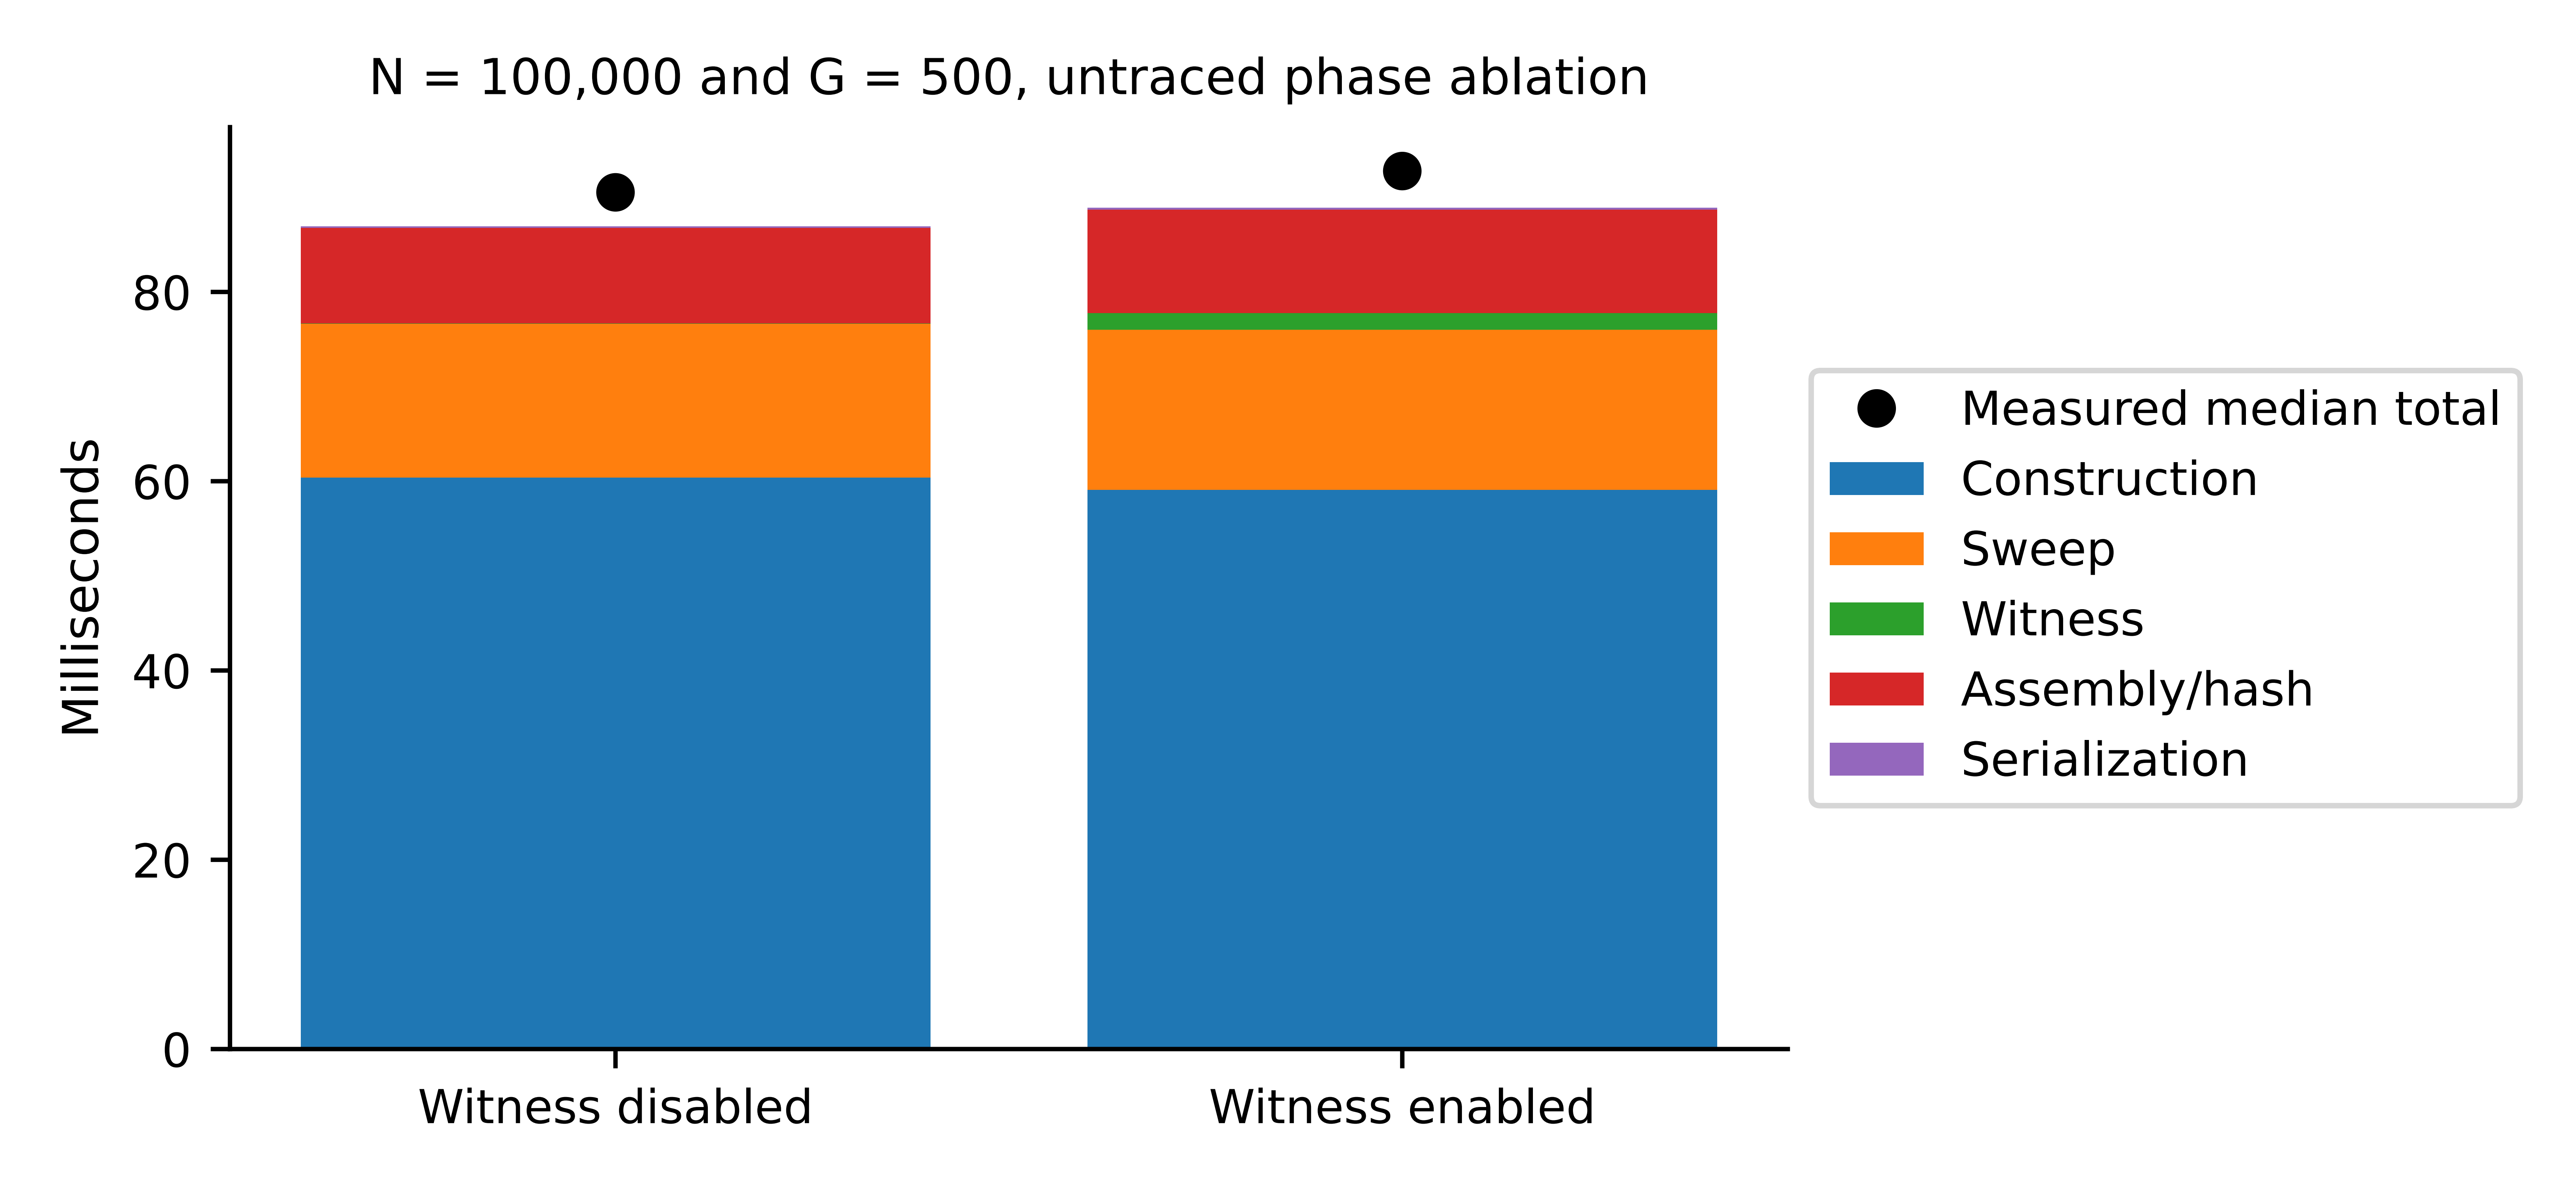
\includegraphics[width=0.88\textwidth]{figures/fig_s1.png}
\caption{Phase medians and measured total. Stacked component medians need not equal the median end to end total}\label{fig:s1}
\end{figure}
\FloatBarrier

End-to-end timings do not identify which part of a certificate computation consumes time. We add a within-invocation ablation with instrumented stage boundaries in the production core. Construction includes input validation, sorting, candidate profiling, exact breakpoint construction and rank summaries. The sweep phase excludes time measured inside witness scans. Witness time records only scans for distinct divergent winning-state pairs. Assembly includes PSC computation and input hashing. Serialization measures JSON encoding outside the core. The certificate returned by an instrumented call is asserted equal to the uninstrumented result on a dedicated test; profiling fields are not inserted into the certificate or used by its logic.

The ablation uses three N/G settings, witness disabled/enabled, and ten rounds per condition, for 60 raw observations. Inputs are prepared outside the timer. Each condition receives a warmup and witness-mode order is randomized within a round. Unlike the original end-to-end traced protocol, this experiment disables tracemalloc. Stage medians below therefore belong to a distinct protocol and should not replace or be pooled with the earlier traced measurements.

See Table~\ref{tab:s8} for untraced phase-ablation medians in milliseconds; component medians need not sum to the median total.

\begin{table}[!htbp]
\caption{Untraced phase-ablation medians in milliseconds; component medians need not sum to the median total}\label{tab:s8}
\centering
\footnotesize
\setlength{\tabcolsep}{2pt}
\renewcommand{\arraystretch}{1.15}
\begin{tabularx}{\textwidth}{@{} >{\raggedright\arraybackslash}p{1.2cm} >{\centering\arraybackslash}X >{\centering\arraybackslash}X >{\centering\arraybackslash}X >{\centering\arraybackslash}X >{\centering\arraybackslash}X >{\centering\arraybackslash}X @{}}
\toprule
\textbf{N} & \textbf{\makecell{Construc-\\tion}} & \textbf{\makecell{Sweep excl.\\witness}} & \textbf{Witness} & \textbf{\makecell{Assembly\\\& hash}} & \textbf{\makecell{Seriali-\\zation}} & \textbf{Total} \\
\midrule
1000 & 0.735 & 0.619 & 0.107 & 0.233 & 0.044 & 1.881 \\
10000 & 5.648 & 4.323 & 0.889 & 1.177 & 0.099 & 13.212 \\
100000 & 59.114 & 16.904 & 1.777 & 10.893 & 0.189 & 92.774 \\
\bottomrule
\end{tabularx}
\end{table}
\FloatBarrier

Values are milliseconds for witness-enabled divergent workloads. Each record also stores the measured end-to-end total and an unattributed residual. The validation checks that phase sums plus that residual equal the same invocation's total, and that witness-disabled calls record zero witness time. Medians of component stages generally need not sum to the median of totals; we do not force that identity or infer witness overhead by subtracting independent medians. The extra clock reads themselves incur overhead, and scheduler variation affects short phases.

The decomposition exposes both sorting/breakpoint work and output/witness work. Witness scans scale with the number of distinct divergent states, not just observation count. A low-cost invariant scan cannot stand in for successful witness construction. Likewise, an efficient policy sweep does not imply a constant-cost independently checkable certificate: hashing, serialization and an external mask-enumeration checker still consume resources. We keep algorithmic asymptotics, measured Python implementation costs, and the slower independent checker as separate claims.


\subsection*{S11 Local CI execution and frequency context}\phantomsection\label{sec:s11}

We execute actual CLI subprocesses for three pipeline representatives, the reference and strict-precision program, three probe modes and three repetitions, then six complete-mode invocations on a separate controlled N=100{,}000/G=500 input. The sixty timed processes are accompanied by three negative CLI checks that require exit 2 for unsupported source. All reference jobs pass and every complete-mode strict-precision job fails as expected. Partial-mode outcomes reflect only their evaluated points.

For the small pipeline representatives, the across-invocation median process time is 449.36 ms and median in-gate time is 10.29 ms. On the separate 100{,}000-row fixture, the corresponding medians are 4292.43 ms and 3891.59 ms. Process time includes Python startup, imports, input loading and report writing; in-gate time excludes startup and includes repeated-determinism checks, candidate masks and reference comparison. They are paired measurements from these invocations, not directly comparable to the traced compact-certificate benchmark or an estimate for a remote runner. Only three repetitions per program at this scale were measured.

This is practical local workflow evidence: CI can distinguish pass, regression and unsupported programs and attach a concrete report. It does not establish an acceptable latency budget for every team, the best testing frequency, remote GitHub execution, or a production SLO. A team could choose checks per commit or per release according to its own case count and latency budget; we make no numerical frequency recommendation from one host. Actual deployment across projects remains an external-validity limitation.


\subsection*{S12 Direct SMT baseline on the same equivalence contract}\phantomsection\label{sec:s12}

Beyond broad capability comparisons, we encode the external threshold-consumer task directly in Z3 \cite{demoura2008z3}. $\alpha$ is a real variable in $[3/10, 9/10]$. A candidate is feasible under the exact linear inequality $\alpha$*n $\le$ k. Candidates are ordered by their fixed (TP,N) priority, and nested if-then-else terms compute the winning selected count. For this same-score task, candidates from both versions belong to one chain of score-prefix memberships, so different winning counts are equivalent to different selected memberships. That reduction does not apply to arbitrary score reorderings; we do not use it for them.

The solver asks whether any policy makes the two winning counts unequal. SAT supplies a rational policy witness; UNSAT asserts full-domain equality for the encoded task. Timeout/unknown is never interpreted as equivalence. We independently re-evaluate each SAT model with direct memberships. The complete partition checker separately emits all interval/endpoint evidence and PSC. Both therefore share a Boolean equivalence contract, while their diagnostic outputs differ. The baseline is our explicit finite SMT encoding using an established solver, not a reproduction of a published threshold-testing tool.

Across 93 variant/input tasks and three repetitions, all 279 solver verdicts agree with partition verification; there are 0 unknown outcomes and every SAT policy is independently checked. Persisted SMT-LIB queries are resolved again by the artifact validator. Median encoding time is 8.222 ms and median solving time is 0.576 ms across those queries. Counts/masks are prepared before these timers. These measurements do not establish a speed ranking against full interval construction with input validation, hashing, witnesses and JSON serialization. The direct SMT results demonstrate that full-domain Boolean comparison is also attainable with a general reasoning engine, narrowing the defensible contribution to the selector-specific contract, complete diagnostics, independently checkable output and scoped integration.


\subsection*{S13 Repeated reuse cost protocol and limits}\phantomsection\label{sec:s13}

See results/v8/reuse\_protocol.json for the predeclared selection and requests, reuse\_raw.csv for 720 chronological observations, reuse\_summary.csv for 144 median/IQR groups, reuse\_query\_plans.json for 2,028 distinct plans and reuse\_outputs/ for every saved method answer. Setup includes certificate construction/JSON/full independent verification or independent mask/SMT preparation. The shared interpolation computation is outside all method timers. Request types, endpoints, batch sizes and all six inputs are retained even when a method is slower. Raw observations and deterministic query answers are separately audited. A crossing is defined only on tested batches 1/8/32/128. No developer study, production-policy inventory or universal amortization bound is claimed.


\subsection*{S14 Full certificate request cost protocol}\phantomsection\label{sec:s14}

We now test whether reuse pays for certificate setup, rather than treating a large query count as a productivity result. Six inputs are fixed before measurement: the upstream int8 fixture, Unix-second int32 fixture, small-int32 control, and seed zero of each pipeline family. These are existing controlled SciPy propagation inputs, not six new projects or production configurations. Two request types use distinct rational singleton policies or width-1/20 windows spread deterministically over $[0.30, 0.90]$, with varying endpoint ownership. Batches contain 1, 8, 32 or 128 requests. The scenarios test computational costs; no application policy-frequency distribution is asserted.

The common output is Boolean existence of a difference plus a rational witness. Direct masks prepare candidate memberships once, then evaluate the requested point or all relevant critical points/open cells for a window, stopping on a difference. Incremental Z3 prepares the independent selected-bitset encoding once per batch and uses push/pop for each request; unknown/timeout fails the study. The certificate route includes construction, a JSON roundtrip and independent full verification once per batch before queries. Its current API materializes intersections before projecting the Boolean answer, so that actual implementation cost remains included. No route memoizes query results; requests within a batch are distinct. All routes reuse the same executed interpolation outputs outside timing. These totals start from frozen score vectors; they exclude common SUT execution, imports, disk I/O and human investigation.

Each case/type has one warmup per method, followed by five fresh setups per batch and method with seeded randomized method order and no allocation tracing. There are 720 timing records, 144 statistical groups and 2,028 distinct case/query plans. All 30,420 method/request answers across methods and repetitions agree, and every reported rational witness is checked against independent selection. These are repeated computational observations, not independent defects or deployment trials. Raw phase costs, query outputs and median/IQR records are retained; medians are not pooled across inputs.

The table reports total median milliseconds (IQR) for batch 128, including setup. The other batch sizes and the separately measured setup/query phases remain in reuse\_summary.csv.

See Table~\ref{tab:s9} for full-certificate batch-128 request costs in milliseconds, shown as median (IQR), including setup.

\begin{table}[!htbp]
\caption{Full-certificate batch-128 request costs in milliseconds, shown as median (IQR), including setup}\label{tab:s9}
\centering
\footnotesize
\setlength{\tabcolsep}{3pt}
\renewcommand{\arraystretch}{1.15}
\begin{tabularx}{\textwidth}{@{} >{\raggedright\arraybackslash}p{2.5cm} >{\centering\arraybackslash}p{1.8cm} >{\centering\arraybackslash}X >{\centering\arraybackslash}X >{\centering\arraybackslash}X @{}}
\toprule
\textbf{Workload} & \textbf{Request} & \textbf{Checked certificate} & \textbf{Direct masks} & \textbf{Incremental Z3} \\
\midrule
Upstream int8 & Point & 9.49 (1.84) & 2.65 (3.24) & 125.92 (9.24) \\
Upstream int8 & Window & 26.04 (1.75) & 18.96 (1.72) & 198.72 (26.04) \\
Unix int32 & Point & 11.47 (5.35) & 3.61 (0.35) & 149.92 (41.33) \\
Unix int32 & Window & 20.02 (5.50) & 15.70 (1.66) & 129.55 (29.31) \\
Small int32 control & Point & 9.26 (1.04) & 3.63 (0.87) & 43.07 (8.67) \\
Small int32 control & Window & 8.12 (1.80) & 15.74 (0.33) & 38.59 (3.91) \\
WDBC seed 0 & Point & 17.45 (2.96) & 5.91 (1.27) & 206.53 (21.52) \\
WDBC seed 0 & Window & 100.67 (34.56) & 22.59 (6.40) & 302.73 (47.63) \\
Digits seed 0 & Point & 72.81 (6.03) & 21.45 (1.89) & 366.95 (61.65) \\
Digits seed 0 & Window & 294.57 (59.74) & 42.72 (19.33) & 424.42 (138.27) \\
RF seed 0 & Point & 27.40 (10.63) & 10.77 (0.15) & 334.45 (35.30) \\
RF seed 0 & Window & 52.09 (4.23) & 21.08 (1.96) & 290.38 (52.00) \\
\bottomrule
\end{tabularx}
\end{table}
\FloatBarrier

At batch 128 the checked certificate is faster than direct masks on 0/6 singleton and 1/6 window inputs; it is faster than this incremental Z3 encoding on 6/6 and 6/6 respectively. Observed sustained crossings against direct masks are Small int32 control / continuous\_window at batch 32. A sustained crossing means the first tested batch with a lower certificate total median at that and every larger tested batch; it is a discrete observed comparison, not an inferred exact threshold, significance test or extrapolation beyond 128 requests. Five repetitions on one host do not establish a population advantage.

The mostly negative comparison against direct masks constrains the practical claim. Reuse alone does not justify building a certificate for a small finite decision set or guarantee an advantage even for continuous windows. A separately checkable, persistable diagnostic object may be required for exact localization or handoff, but this experiment does not monetize that requirement or measure a developer's debugging time. It measures a computational tradeoff against specified implementations, including a reused solver, and leaves industrial policies, human triage benefit and superiority over an independently optimized parametric tool unresolved.


\subsection*{S15 Boolean API study and comparison panels}\phantomsection\label{sec:s15}

The exact protocol is results/v9/boolean\_protocol.json. Both certificate routes pay construction, JSON roundtrip and the same independent full verification; the indexed route also pays copying/freezing/index construction. This is the assurance-matched API panel. Direct masks and incremental Z3 answer the same Boolean question without emitting/checking a complete diagnostic object, so four-route totals are a separate request-cost panel with unequal evidence obligations. The original six inputs and 2,028 plans are reused: 960 timing records, 192 groups and 40,560 repeated method answers are not new workloads or defects. Full per-phase medians/IQRs and raw observations are retained. A descriptive speed ratio is not a statistical or deployment guarantee. BOOLEAN\_QUERY\_AND\_ASSURANCE.md gives component-merging/endpoint reasoning, asymptotic scope and refusal behavior.


\subsection*{S16 Detailed production and larger candidate costs}\phantomsection\label{sec:s16}

Main Section 2.5 defines the timing boundaries and Main Section 3.3 reports the central comparisons. The tables below retain all detailed conditions moved from the earlier Main reading copy.

See Table~\ref{tab:s10} for traced certificate-production cost by scale, workload and witness mode; medians and IQRs remain within each condition.

\begin{table}[!htbp]
\caption{Traced certificate-production cost by scale, workload and witness mode; medians and IQRs remain within each condition}\label{tab:s10}
\centering
\footnotesize
\setlength{\tabcolsep}{1.5pt}
\renewcommand{\arraystretch}{1.15}
\begin{tabularx}{\textwidth}{@{} >{\raggedright\arraybackslash}p{1.0cm} >{\centering\arraybackslash}p{1.5cm} >{\centering\arraybackslash}p{1.6cm} >{\centering\arraybackslash}p{1.3cm} >{\centering\arraybackslash}X >{\centering\arraybackslash}X >{\centering\arraybackslash}X >{\centering\arraybackslash}X @{}}
\toprule
\textbf{N} & \textbf{\makecell{G old\\(bins)}} & \textbf{Workload} & \textbf{\makecell{Witness\\enabled}} & \textbf{\makecell{Median\\ms}} & \textbf{\makecell{IQR\\ms}} & \textbf{\makecell{Peak\\MiB}} & \textbf{\makecell{Witness\\cells}} \\
\midrule
1000 & 20 & divergent & False & 9.55 & 1.53 & 0.10 & 0.0 \\
1000 & 20 & divergent & True & 8.26 & 1.55 & 0.10 & 4.0 \\
1000 & 20 & invariant & False & 4.81 & 1.05 & 0.09 & 0.0 \\
1000 & 20 & invariant & True & 4.99 & 0.84 & 0.09 & 0.0 \\
10000 & 100 & divergent & False & 62.46 & 14.70 & 1.00 & 0.0 \\
10000 & 100 & divergent & True & 63.02 & 22.87 & 1.00 & 29.0 \\
10000 & 100 & invariant & False & 35.65 & 2.15 & 0.91 & 0.0 \\
10000 & 100 & invariant & True & 34.97 & 1.71 & 0.91 & 0.0 \\
100000 & 500 & divergent & False & 520.59 & 120.04 & 9.22 & 0.0 \\
100000 & 500 & divergent & True & 528.06 & 40.73 & 9.24 & 111.0 \\
100000 & 500 & invariant & False & 368.19 & 103.85 & 8.80 & 0.0 \\
100000 & 500 & invariant & True & 341.13 & 60.75 & 8.80 & 0.0 \\
\bottomrule
\end{tabularx}
\end{table}
\FloatBarrier

All rows use ten measured repetitions after warmup on one Windows host, Python 3.12.10/NumPy 2.3.5, with randomized mode order, tracemalloc enabled and JSON serialization included. Peak is auxiliary MiB with preallocated inputs excluded, not process RSS. The N=100{,}000 divergent witness-enabled median is 528.06 ms (IQR 40.73), emitting 111 witness-bearing state cells; the corresponding witness-disabled median is 520.59 ms (IQR 120.04). These runs activate witness construction, unlike the earlier one-policy invariant guard benchmark. No significance, independence, universal speed advantage, or direct cross-protocol latency ratio is asserted. Raw chronological records and exact seeds/generation code are included.

The eight external affected/fixed tasks remain a separate check and still agree. We add a prespecified factorial design: N in {1{,}000,10{,}000,100{,}000}, G in {10,30,90}, and no, one-middle, or alternating candidate omission. Scores form G tied groups with gradually decreasing group-positive proportions; fixed-seed permutations remove dependence on row order. These designed families yield 0--39 divergent components. They are controlled tasks, not new upstream defects or independent deployments. Every one of the 27 tasks is retained, including empty-divergence controls.

Five repetitions per method/task, with randomized method order inside each repetition, produce 270 timing records and 54 saved certificates. Both methods receive the same candidate family, regenerate counts/masks during each timed preparation, emit the same diagnostic JSON and invoke the same independent region checker. All complete outputs agree and every saved certificate is replayed. Preparation, producer plus serialization, checker, total checked cost, candidate counts, exact critical-point count, divergent components, probes, bytes and solver calls are retained separately. Thus input-size effects are not inferred from a preparation-excluded timer alone.

The previous G$\le$90 factorial is extended with six additional prespecified tasks at N=10{,}000, G in {250,500} and the same none/one/alternating omission patterns. Both algorithms still produce identical complete diagnostics. Three repetitions per method, randomized within each replicate, yield 36 raw timing records and twelve independently replayed certificates. No task is dropped for being unfavorable. Residual UNSAT is required for SMT completion; unknown or timeout would prevent certification.

See Table~\ref{tab:s11} for complete diagnostic comparison for larger candidate counts at N = 10{,}000; three repetitions per method.

\begin{table}[!htbp]
\caption{Complete diagnostic comparison for larger candidate counts at N = 10{,}000; three repetitions per method}\label{tab:s11}
\centering
\footnotesize
\setlength{\tabcolsep}{3pt}
\renewcommand{\arraystretch}{1.15}
\begin{tabularx}{\textwidth}{@{} >{\raggedright\arraybackslash}p{2.5cm} >{\centering\arraybackslash}p{2cm} >{\centering\arraybackslash}p{2cm} >{\centering\arraybackslash}X >{\centering\arraybackslash}X @{}}
\toprule
\textbf{G / omission} & \textbf{Critical points} & \textbf{Components} & \textbf{Partition total ms} & \textbf{SMT total ms} \\
\midrule
250 / none & 215 & 0 & 986.40 & 797.28 \\
250 / one & 215 & 1 & 735.13 & 918.14 \\
250 / alternating & 215 & 107 & 973.93 & 3649.18 \\
500 / none & 430 & 0 & 3618.14 & 2268.31 \\
500 / one & 430 & 1 & 3993.99 & 4715.14 \\
500 / alternating & 430 & 215 & 5291.80 & 21336.96 \\
\bottomrule
\end{tabularx}
\end{table}
\FloatBarrier

Totals include fresh candidate preparation, complete region/witness production plus JSON and the same region checker. The new cases reach 430 critical points and 215 divergent components. Three repetitions are descriptive and are not pooled with the older five-repetition protocol. The prepared-membership region checker is distinct from the streaming consumer for the core certificate schema. These results extend the evaluated candidate range, but do not establish asymptotic superiority, a deployment SLO, or a win over an independently optimized AllSMT implementation. The baseline remains our direct Z3 encoding; modern enumeration methods \cite{spallitta2025disjoint} retain capabilities and optimizations this study does not benchmark.


\subsection*{S17 Implementation and operational details}\phantomsection\label{sec:s17}

The certificate records selector contracts, input SHA-256, domain, all critical fractions, state intervals, membership counts, an equality verdict, optional observation witness and exact PSC. It does not store all selected IDs; the original input arrays are needed for verification. The independent verifier constructs actual threshold masks and integer bitsets, independently derives critical values, and checks coverage, winners, witnesses, counts and PSC. It shares the mathematical contract, but not the production heap or rank comparator.

The unstreamed materialized consumer materializes all Boolean threshold masks in memory ($\mathcal{O}(NG)$ space). The streaming consumer instead imports neither the producer nor the unstreamed checker, counts one threshold mask at a time in $\mathcal{O}(1)$ simultaneously active masks, and retains exact feasibility ratios, actual TP/N counts and candidate descriptors. A reverse suffix-maximum table over sorted ratios supplies fixed-priority winners by exact bisection. Current winning memberships are reconstructed and packed directly from the inputs; no all-candidate bitset cache or production rank-containment comparator is used.

The suffix winner argument is direct: feasible candidates form a suffix (lower bound for inclusive feasibility, upper bound for strict feasibility), and reverse induction computes that suffix's maximum fixed priority. Independent critical-point construction, ordered certificate coverage and endpoint ownership then justify checking all atom representatives. A forward cell cursor validates each probe; actual bitsets validate equality, witness IDs/memberships and changed-row counts. Exact divergent length and PSC are independently recomputed. Detailed lemmas and conditional soundness are in Online Resource~1 (Section~S1) and STREAMING\_CHECKER\_AND\_FLOAT\_CUT\_PROOFS.md. These are mathematical arguments plus tests, not a machine-checked proof or independent human replication.

The consumer uses O(N+G+K+C) auxiliary descriptors/probes and current-mask storage, excluding arbitrary-precision operand sizes, for K critical values and C certificate cells. Direct counting and winner reconstruction retain worst-case $\mathcal{O}(NG)$ work; split-tie ordering adds $\mathcal{O}(N \log N)$, with ratio/query/probe sorting costs stated in the proof supplement. In particular, G=N can still be quadratic. Suffix maxima, bisection and streaming are established techniques \cite{mcconnell2011certifying}, not new general primitives.

A rational-domain query interface operates after independent certificate verification. Finite sets and decimal lattices return affected counts; intervals return exact intersected cells. All retain endpoint ownership and a rational witness when affected. Tampered inputs, out-of-domain requests and binary64 queries sent to the rational interface are refused. This checks the declared domain on the fixed inputs; it does not infer a production requirement.

We add VerifiedBooleanIndex. Its constructor copies and independently verifies the complete input-bound certificate, merges adjacent unequal cells only when their shared endpoint is included, and freezes a rational interval index with the checked input digest. A matching singleton hole between two open unequal regions is preserved. A query searches the ordered component endpoints and returns only Boolean existence plus one rational policy witness; it never constructs the full intersection list. Finite-set and decimal-lattice queries retain explicit rational semantics, domain validation and endpoint ownership. Counts and complete intersected regions remain available from the original API. This is an application of established interval union and binary search, not new parameter-region theory.

After construction, interval and singleton queries take O(log C) rational comparisons plus bounded candidate checks over C maximal components. A finite set performs point queries after validation/deduplication. A lattice may scan O(C) components before finding a lattice member or establishing absence, so it has no logarithmic worst-case claim. Construction and full independent checking remain separate costs; arbitrary-precision operands matter. BOOLEAN\_QUERY\_AND\_ASSURANCE.md gives the reasoning and exact interface. Four targeted tests exercise zero-measure divergence, a matching singleton hole, input tamper/immutable reuse and unsupported domains.

policy\_cli.py loads aligned NPZ arrays and writes a certificate after independent verification. --fail-on-divergence yields exit code 1 and a concrete interval/row witness. The pytest assertion wrapper reports the first divergent state; equality returns a certificate. An example GitHub Actions workflow runs tests and artifact verification locally configured for this folder. The workflow is supplied as a template; it has not been uploaded or executed on a remote CI service.

Online Resource~1 (Section~S4) documents unsupported-source fixtures, runtime refusals and CLI exit semantics. Refusal is never interpreted as equivalence.

For RQ1, we test the finite contract by exhaustive and randomized comparisons, independently replay certificates, check recorded grid outcomes and retain explicit endpoint/tamper cases. For RQ2, the measured outcomes are selected-ID divergence, executable nonconformance and baseline detections within each separately defined corpus. Snapshot probes use $\alpha$ = 0.50; the grid uses thirteen targets from 0.30 through 0.90. Corpus denominators and identity violations are never pooled with upstream defect counts.

Snapshot and grid tests observe actual configured mutant outputs. B4/current guard observe score arrays and do not inspect changed selector code. Their aggregate scores therefore have different scope. An exact certificate is configured with the mutant's declared finite contract; applying it to arbitrary real software requires a faithful adapter. Detection of the declared fault model does not certify that adapter automatically.

Correctness tests enumerate 4,680 binary-score/label pairs up to N=4 and 6,174 ternary-score cases up to N=3 (10{,}854 total), plus 1{,}000 seeded randomized variants. Additional pytest checks cover endpoint-only changes, invalid values/shapes, aligned identities, abstention, certificate tampering and actionable CI failures. These are finite implementation checks, not a proof of universal program correctness.

For RQ3, we measure elapsed time, within-task median/IQR and separately defined auxiliary memory. The traced producer protocol includes certificate construction and JSON serialization, ten repetitions per condition after warmup, randomized witness-mode order and one Windows host with Python 3.12.10/NumPy 2.3.5. Preallocated inputs are excluded from auxiliary MiB, which is not process RSS. The preparation-matched study in Online Resource~1 (Section~S9) and untraced ablation in Online Resource~1 (Section~S10) retain distinct instrumentation; their medians are not pooled with this protocol.

The complete-region comparator uses a direct Z3 encoding \cite{demoura2008z3}, not an independently optimized AllSMT implementation. Both routes must return maximal divergent components, exact endpoint ownership and PSC, a Boolean equivalence verdict and an existential policy/row witness per component. SMT expands each QF\_LRA model to its complete feasibility-predicate cell and blocks that cell; residual UNSAT is required for completion. Unknown/timeout prevents certification. General predicate enumeration is established \cite{mathsat_api,spallitta2025disjoint}; the comparison measures implementations under a common diagnostic output contract.

The smaller-candidate factorial crosses N in {1{,}000,10{,}000,100{,}000}, G in {10,30,90} and three omission patterns: none, one middle group or alternating groups. Scores form tied groups with gradually decreasing positive proportions and fixed-seed row permutations. All 27 tasks, including empty-divergence controls, are retained. Five repetitions per method/task randomize method order. Both routes regenerate counts/masks during timed preparation, serialize the diagnostic JSON and invoke the same region checker. Preparation, production/serialization, checking and total cost are recorded separately. Eight earlier external tasks remain a separate check. A larger-candidate extension uses N = 10{,}000, G in {250,500}, the same omission patterns and three randomized repetitions per method; these protocols are not pooled.

The paired experiment regenerates the same six N/G fixtures as the earlier checker study, prepares an identical certificate/payload outside timing, warms up both consumers, and randomizes their order within each of five repetitions. JSON parsing is recorded separately. A sixth invocation per consumer/group traces memory independently. The sixty untraced timing records and twelve separate memory records are never pooled. Each paired comparison uses identical inputs, policies, coverage, hash and witness obligations; these are not ratios against the differently instrumented producer benchmark.

For RQ4, we compare rational-reference and binary64-interface outcomes and intersect exact divergent components with declared policy sets. Quantiles use exact fractions and linear interpolation, with conversion only for display. Four rational decimal lattices on $[0.30, 0.90]$ are intersected algebraically using integer bounds and endpoint ownership. Representable-binary64 probes are embedded by their exact integer ratios, so they are not substituted for decimal targets. The 36 SciPy defect-study workloads are each assessed under eight predeclared finite, lattice and interval scenarios. Direct masks use cached executed interpolation outputs; an independent selected-bitset Z3 encoding \cite{demoura2008z3} checks existence, with integer lattice indices or real interval policies. SAT witnesses are checked by direct selection; unknown/timeout aborts the comparison.

The reuse protocols distinguish two certificate APIs from direct-mask and incremental-Z3 request costs. Both certificate APIs pay construction, JSON roundtrip and the same independent full verification; the Boolean route also pays copying, merging, freezing and indexing. Direct masks and Z3 do not emit/check a complete diagnostic certificate. Table~\ref{tab:s12} makes the evidence obligations explicit; checking a positive witness alone does not independently establish a direct negative result or an UNSAT proof.

The paired Boolean API study reuses six existing inputs, two request types, distinct rational point/window plans and batch sizes 1/8/32/128. One warmup per case/type/method precedes five fresh setups per batch/method, with seeded randomized order. Common interpolation, imports, disk I/O and human activity are excluded. Requests within a batch differ and no result memoization is used. Phase timings and total costs remain separate; medians are computed within each condition. The separate 720-record full-certificate request-cost protocol is retained separately in Online Resource~1 (Section~S14); it is not pooled with the paired API study.

This document revision used OpenAI Codex (OpenAI) for evidence-validation and visualization-authoring scripts. Figures are deterministic plots of the recorded research results; typography is adjusted without changing the underlying measurements. The research artifact also includes assistant-generated code and prose. Its computational scripts, raw measurements and independent checker outputs remain available; computational checks alone do not establish independent human review or replication.

\begin{table}[!htbp]
\caption{Evidence-production and independent-checking obligations of the four Boolean query routes}\label{tab:s12}
\centering
\footnotesize
\setlength{\tabcolsep}{2.5pt}
\renewcommand{\arraystretch}{1.15}
\begin{tabularx}{\textwidth}{@{} >{\raggedright\arraybackslash}p{3cm} >{\centering\arraybackslash}p{2.2cm} >{\centering\arraybackslash}p{2.2cm} >{\raggedright\arraybackslash}X @{}}
\toprule
\textbf{Route} & \textbf{Complete certificate produced} & \textbf{Independent full certificate check} & \textbf{Query operation used here} \\
\midrule
Full certificate API & Yes & Yes & Full API, then Boolean/witness projection \\
Boolean certificate API & Yes & Yes, with the same checker & Indexed Boolean/witness lookup \\
Direct masks & No persisted complete certificate & No certificate to check & Exact masks/critical-cell evaluation \\
Incremental Z3 & No complete diagnostic certificate & No exported proof/\allowbreak certificate checked & SAT/UNSAT with rational SAT witness \\
\bottomrule
\end{tabularx}
\end{table}
\FloatBarrier

\begin{table}[!htbp]
\caption{Batch-128 total median query cost in milliseconds, including route-specific setup, on the existing six inputs}\label{tab:s13}
\centering
\footnotesize
\setlength{\tabcolsep}{2.5pt}
\renewcommand{\arraystretch}{1.15}
\begin{tabularx}{\textwidth}{@{} >{\raggedright\arraybackslash}p{2.4cm} >{\centering\arraybackslash}p{1.6cm} >{\centering\arraybackslash}X >{\centering\arraybackslash}X >{\centering\arraybackslash}X >{\centering\arraybackslash}X @{}}
\toprule
\textbf{Workload} & \textbf{Request} & \textbf{Full certificate} & \textbf{Boolean certificate} & \textbf{Direct masks} & \textbf{Incremental Z3} \\
\midrule
Upstream int8 & Point & 3.41 & 2.62 & 1.75 & 45.44 \\
Upstream int8 & Window & 11.23 & 6.03 & 10.50 & 74.22 \\
Unix int32 & Point & 7.16 & 4.89 & 2.06 & 91.57 \\
Unix int32 & Window & 7.84 & 2.61 & 7.63 & 56.65 \\
Small int32 control & Point & 3.59 & 3.68 & 1.95 & 32.11 \\
Small int32 control & Window & 5.52 & 3.26 & 9.53 & 24.25 \\
WDBC seed 0 & Point & 15.01 & 7.59 & 2.77 & 111.84 \\
WDBC seed 0 & Window & 27.29 & 5.70 & 11.96 & 84.00 \\
Digits seed 0 & Point & 43.92 & 10.80 & 19.31 & 189.20 \\
Digits seed 0 & Window & 177.87 & 16.38 & 32.18 & 164.59 \\
RF seed 0 & Point & 11.40 & 6.01 & 6.05 & 163.68 \\
RF seed 0 & Window & 21.06 & 5.93 & 10.75 & 129.52 \\
\bottomrule
\end{tabularx}
\end{table}
\FloatBarrier

The paired API protocol yields 960 timing records and 192 median/IQR groups. Its 2,028 existing case/query plans produce 40,560 repeated method answers across four routes and five repetitions; all agree and saved rational witnesses are independently checked. These repetitions do not enlarge the empirical defect corpus. Table~\ref{tab:s13} reports batch-128 total medians, including each route's setup; phase medians, IQRs and other batches remain in the raw records.

In the assurance-matched panel, Boolean lookup lowers the query-phase median in 12/12 batch-128 combinations, by 2.06--35.39 times. Including all setup, its total median is lower in 11/12 combinations; the remaining cases are retained. Thus part of the full-certificate route's cost came from its output construction, while construction and independent certificate checking still have a price. These are descriptive paired medians on one host, not a statistical significance result or a universal speed guarantee.

In the four-route request-cost panel, the Boolean route has lower total medians than direct masks for 2/6 point and 6/6 window inputs, and than this incremental Z3 encoding for 6/6 and 6/6. Those comparisons have the unequal obligations shown above and are not a ranking of equal verification guarantees or optimized external tools. Direct checking remains a valid simpler choice for a small finite allowed set. Computational reuse results do not measure developer debugging time, production policy requirements, institutional adoption or deployment break-even. The contribution remains exact diagnosis and checkable evidence with explicit interface and cost boundaries.

RQ4 demonstrates that declared domains can change the diagnostic answer and that API output work affects measured reuse costs. It does not establish which domains users require or a general break-even point for creating certificates.


\subsection*{S17.3 Empirical comparison with boundary-aware direct testing baseline}\phantomsection\label{sec:s17_3}

A natural question in software testing is whether the proposed certificate-based framework provides a genuine empirical advantage over a simpler alternative: \textit{boundary-aware direct probing}. Under this baseline, rather than constructing a certificate or running a sweep, a test harness derives the complete set of critical feasibility ratios $B = \{L, H\} \cup \{k/n \in (L, H)\}$ (where $K = |B|$ is the total number of critical boundary values including domain endpoints $L$ and $H$) and intermediate open-atom midpoints $(b_{i-1} + b_i)/2$. The canonical partition of $[L, H]$ consists of $K$ boundary singletons and $K-1$ open interval atoms, yielding exactly $2K-1$ elementary policy atoms and probe points. The baseline then repeatedly evaluates candidate sets across all $2K-1$ probe points.

To isolate algorithmic differences fairly, Table~\ref{tab:s13_boundary} presents a phase-level benchmark on four representative cohorts under invariant conditions ($N \in \{143, 450, 600, 37{,}471\}$). Both methods receive identical preprocessed candidate tables and evaluate the exact same $2K-1$ critical policy atoms. Timings reflect medians and interquartile ranges (IQR) across five randomized repetitions under Python 3.11 on Windows x86\_64 (measured via \texttt{perf\_counter\_ns}; raw records in \texttt{results/phase\_benchmark\_raw.csv} and summary in \texttt{results/phase\_benchmark\_summary.json}, generated by \texttt{run\_phase\_benchmark.py}).

\begin{enumerate}
\item \textbf{Repeated candidate-scanning cost vs. monotone heap sweep:} Direct boundary probing scans candidate descriptors across all $2K-1$ probes, incurring a cost bounded by $\mathcal{O}((K+C) \cdot G)$. In candidate-dense settings where $G = \Theta(N)$ (e.g., Digits with $N=450, G=450, K=106$), direct probing core requires $75.24\text{ ms}$ (IQR $10.20$), whereas the monotone heap sweep requires only $1.45\text{ ms}$ (IQR $0.20$)---a $52.0\times$ core algorithmic speedup ($10.9\times$ on Generated RF). When $G \ll N$ (e.g., Simulated Cold-Chain with $N=37{,}471, G=87$), sweep core remains $4.8\times$ faster ($0.14\text{ ms}$ vs. $0.70\text{ ms}$). To illustrate the lifecycle impact of these obligations under assumed shared packaging costs, if direct probing were extended to produce the same certificate schema (witness extraction and input hashing, estimated at $2.32\text{ ms}$ on Digits by subtracting sweep core from full producer median) and checked via the same streaming verifier ($11.19\text{ ms}$), the resulting illustrative component-based latency estimate would be $88.75\text{ ms}$ vs. $14.96\text{ ms}$ (an estimated $5.93\times$ end-to-end ratio). We emphasize that this $5.93\times$ figure is an analytical component-based estimate under assumed shared overheads rather than a separately measured paired end-to-end benchmark; the primary measured empirical speedup remains the $52.0\times$ core sweep speedup in Table~\ref{tab:s13_boundary}. Decomposing the full lifecycle into $T_{\text{total}} = T_{\text{preparation}} + T_{\text{production}} + T_{\text{verification}} + T_{\text{query}}$ illustrates the component-level cost tradeoffs and workload-dependent conditions under which certificate reuse may become advantageous under the evaluated protocols, confirming that the $52.0\times$ core algorithmic speedup does not apply uniformly to the complete end-to-end certification lifecycle. Moreover, while theoretical bounds show asymptotic efficiency, these empirical measurements describe the four evaluated configurations and do not establish universal scaling across arbitrary unmeasured $(N, G, K)$ combinations.
\item \textbf{Ephemeral verdict versus certifying auditability:} The evaluated stateless direct probing baseline produces only a transient Boolean verdict. In contrast, the proposed method generates an input-bound diagnostic certificate containing exact boundaries, PSC, and observation-level witnesses, independently verifiable against the original input arrays.
\item \textbf{Streaming consumption versus full-mask materialization:} A materialized-mask implementation of direct probing verification may retain $\mathcal{O}(NG)$ Boolean storage, whereas the proposed consumer reconstructs threshold masks sequentially and avoids retaining all candidate masks simultaneously (retaining only a constant number of simultaneously active masks, with $\mathcal{O}(N + G + K + C)$ auxiliary descriptor storage). Independent verification completes in $11.19\text{ ms}$ on Digits and $24.85\text{ ms}$ on Simulated Cold-Chain.
\item \textbf{Query lattice reuse and break-even context:} When operating conditions shift or callers query sub-domains, the stateless direct probing baseline must repeat all $2K-1$ candidate evaluations from scratch. In contrast, once verified, the certificate enables exact sub-domain interval and point queries in approximately $17\text{--}28\ \mu\text{s}$ ($16.7\text{--}27.7\ \mu\text{s}$ across the four evaluated fixtures in Table~\ref{tab:s13_boundary}, $\mathcal{O}(\log(M+1))$). As shown in the comprehensive reuse evaluation (Sections~S13--S15), this query-level advantage does not make the certificate universally faster for every deployment scenario: for isolated, one-off queries with small batch sizes, stateless evaluation avoids certificate setup overhead and achieves lower total latency. The certificate-based route may become advantageous when query batches amortize setup costs, or when independent verification and persistent auditability are explicit application requirements.
\end{enumerate}

\begin{table}[!htbp]
\caption{Phase-level benchmark comparison between Boundary-Aware Direct Probing and the proposed framework across four benchmark cohorts under invariant conditions (five repetitions; median and IQR; Simulated Cold-Chain models $N=37{,}471$ telemetry readings with deterministic rule-based $2\text{--}8^\circ\text{C}$ safe-window excursion criteria)}\label{tab:s13_boundary}
\centering
\footnotesize
\setlength{\tabcolsep}{3pt}
\renewcommand{\arraystretch}{1.15}
\resizebox{\textwidth}{!}{%
\begin{tabular}{@{}lrrrrrrrr@{}}
\toprule
\textbf{Workload cohort} & \textbf{$N$} & \textbf{$G$} & \textbf{$K$} & \textbf{\makecell{Direct probing\\core ms (IQR)}} & \textbf{\makecell{Sweep producer\\core ms (IQR)}} & \textbf{\makecell{Core\\speedup}} & \textbf{\makecell{Producer full\\cert ms (IQR)}} & \textbf{\makecell{Streaming check\\ms (IQR)}} \\
\midrule
WDBC & 143 & 15 & 8 & 0.33 (0.02) & 0.09 (0.03) & 3.6$\times$ & 0.47 (0.17) & 0.76 (0.10) \\
Digits & 450 & 450 & 106 & 75.24 (10.20) & 1.45 (0.20) & 52.0$\times$ & 3.77 (2.01) & 11.19 (0.80) \\
Generated RF & 600 & 54 & 33 & 3.20 (0.75) & 0.29 (0.02) & 10.9$\times$ & 1.01 (0.01) & 2.25 (0.51) \\
Simulated Cold-Chain & 37{,}471 & 87 & 6 & 0.70 (0.05) & 0.14 (0.01) & 4.8$\times$ & 11.94 (1.14) & 24.85 (1.61) \\
\bottomrule
\end{tabular}%
}
\end{table}
\FloatBarrier

\begin{figure}[!htbp]
\centering
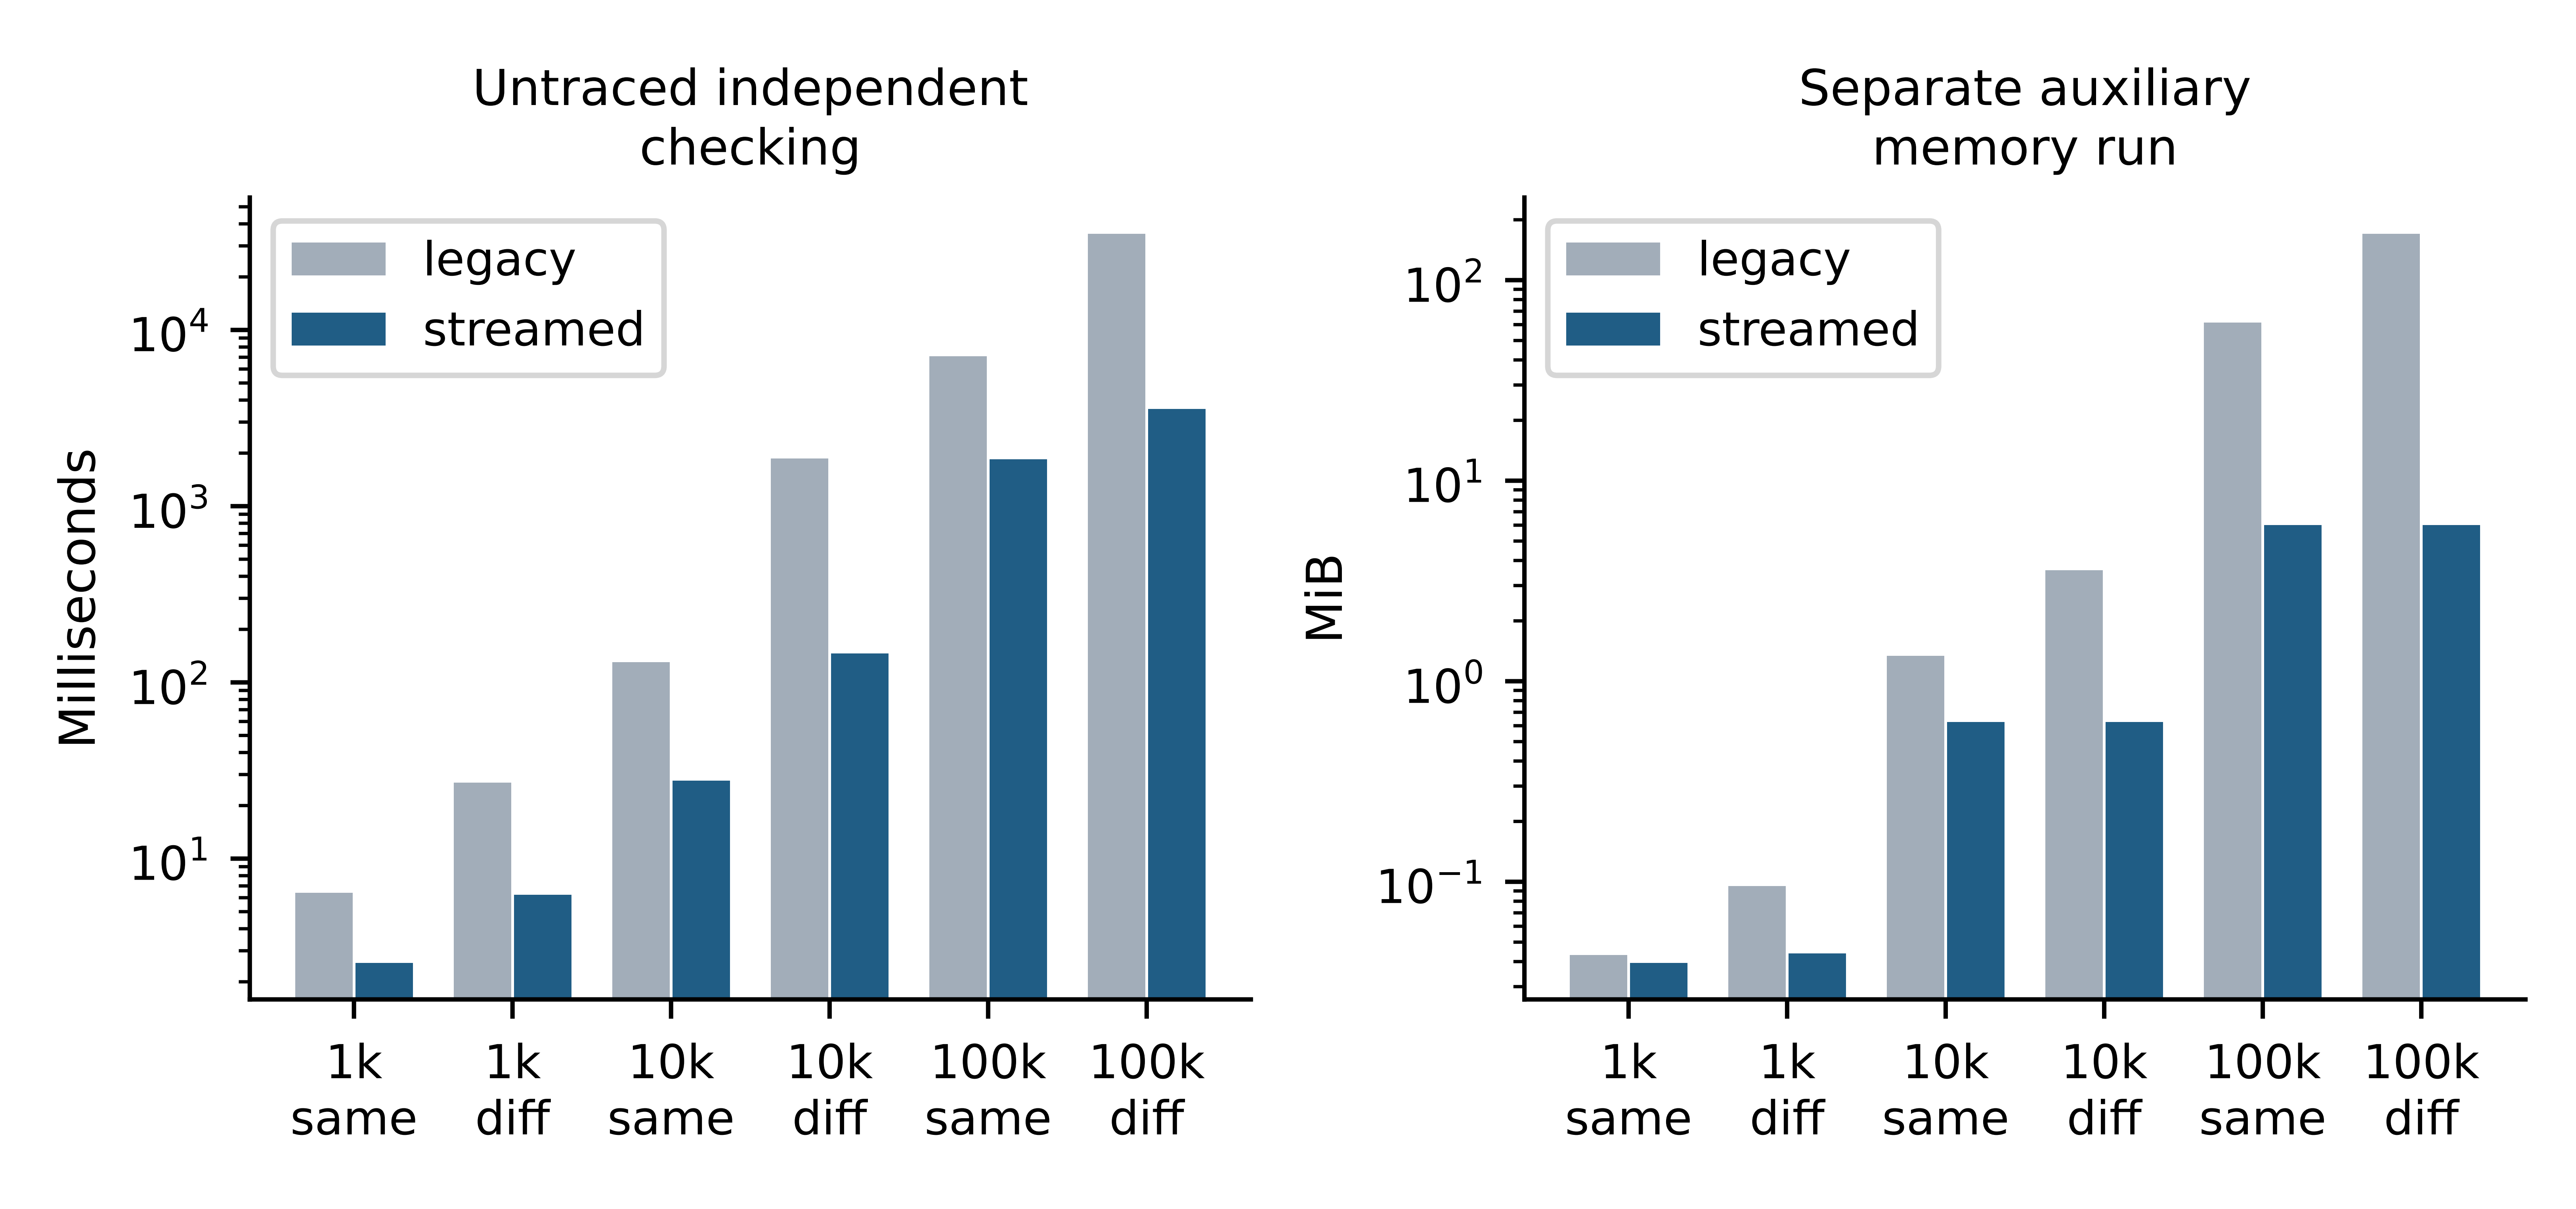
\includegraphics[width=0.76\textwidth]{figures/fig_s2.png}
\caption{Paired independent-consumer timing and separately traced auxiliary memory on identical fixtures. Axes are logarithmic; these are separate measurement protocols}\label{fig:s2}
\end{figure}
\FloatBarrier


\section*{D Reproducibility and source integrity}\phantomsection


\subsection*{S18 Reproduction and assurance levels}\phantomsection\label{sec:s18}

The original standalone failure arose because the experiment driver read a historical 255-row grid CSV from a neighboring submission tree. The corrected driver reads a bundled inputs/historical/ copy and asserts its checksum from the input manifest before any comparison. Default run\_all.py works from frozen arrays within the extracted artifact; it does not refit models, reinstall dependency versions or need the old submission directory. Optional model refitting is a separate command with its source-data requirements documented. The distinction prevents the term “standalone” from silently including unbundled training assets.

Assurance has several layers. Unit/exhaustive tests validate finite implementations on small and randomized cases. The independent certificate checker reconstructs actual threshold masks on all stored application and declared-mutant certificates. The program adapter calls a separate executable and checks the unchanged reference contract under an explicit guard-coverage restriction. Fresh version workers establish what two actual dependency binaries computed. Checksummed packaging and a clean extraction run test delivery rather than mathematical correctness. None of these layers, alone or together, establishes authenticity of upstream measurements, population model quality, a universally correct verifier or an industrial real-bug detection rate.

Previous internal build archives from development are retained for historical traceability; the current released archive \texttt{Reproducibility\_Artifact.zip} is the self-contained evaluation package. Revised raw records are regenerated rather than mixed with old timings. Source snapshots bind the producer used for those records. A final manifest is generated after documents, evidence and reports have been assembled. The clean-run report names the extracted path, absence of neighboring SUBMISSION\_PACKAGE, interpreter, stage exit codes and resulting logical summaries. It is a local clean reproduction, not independent human replication. A broader upstream-confirmed bug corpus and prospective deployment study remain work outside this revision; two isolated-source upstream defect case studies are now included.


\subsection*{S19 Source provenance and study scope}\phantomsection\label{sec:s19}

The scientific implementations and the 33-stage protocol are bound in \texttt{provenance/\allowbreak v9\_\allowbreak science\_\allowbreak source\_\allowbreak hashes.json}. The manuscript bibliography contains 29 references, including scholarly publications, software documentation, standards, and upstream issue/PR records. The artifact retains source hashes, frozen evaluation inputs and detached execution records. These records document the implementation and evaluation of the present study. Revision history is retained in \texttt{docs/\allowbreak ARTIFACT\_\allowbreak CHANGELOG.md} alongside the current manuscript sources.


\subsection*{S20 Cross platform source snapshot integrity}\phantomsection\label{sec:s20}

Generated mutant and refusal-fixture Python sources use explicit UTF-8 bytes and LF newlines, followed by byte-hash verification. Execution-source copies retain actual source bytes. The default 33-stage chain is self-contained; revision-named files are cumulative study components, not dependencies on old release ZIPs. Historical source-binding counts and repairs are documented in the artifact changelog. Native Linux execution has not been claimed.


\subsection*{S21 Reproduction entry point and result traceability}\phantomsection\label{sec:s21}

The computational authority is the exact frozen artifact paired with its detached execution report. Reproducibility\_Artifact.zip has SHA-256 \texttt{\seqsplit{98cfc7ec8498214a79717480e5a8be83707cc4244296fe3cb589a329dc4fa8aa}}; Reproducibility\_Evidence.zip has SHA-256 \texttt{\seqsplit{0e30a95b24d08cde64e68778d0eba1e211af97e68fe950ff76f021a22793115b}}. ARTIFACT\_MANIFEST.json covers 3,500 artifact payload files. EVIDENCE\_MANIFEST.json covers 43 detached payload files, excluding itself. The two archives are accompanying reviewer files; a public URL/DOI remains an author item.

For default reproduction, create or activate a Python 3.13.18 environment, extract the artifact into a clean directory, and run the following commands from that root. Dependency specifications include NumPy 2.3.5, SciPy 1.18.1, scikit-learn 1.9.1, pytest 9.2.0, z3-solver 5.3.3.0 and the bundled eval-toolkit 1.12.0 wheel. The exact installed package inventory and Windows host are recorded in RELEASE\_VERIFICATION.json. Historical reading-copy timings include a Python 3.12.10 producer protocol; those are separate measurement records rather than a claim that every benchmark used the final execution interpreter.

\begin{verbatim}
python -m pip install -r requirements.txt
python run_all.py
\end{verbatim}
The single entry point runs 33 stages. Expected logical outcomes include 42 passing core tests, 18 separate upstream tests, 98 input bindings, 428 application/mutation certificates, 41{,}348 critical/open-cell probes, 360 configured mutation/control records, 183 configured policy divergences, and 136 executed nonconforming runs. The recorded full execution took 2,345.58 seconds (about 39.1 minutes) on one Windows host. This duration is descriptive; reruns need not reproduce timing, memory or all output bytes.

Default frozen-input reproduction rebuilds comparisons, certificates, generated local programs and computational measurements from supplied arrays. It does not retrain models or install two historical SciPy versions in the same interpreter. Fresh binary re-execution needs separate environments containing the specified dependency versions and the documented version\_worker.py commands; each worker checks its loaded version. Optional model retraining uses the documented source-data/preparation route and additional assets, and is not a prerequisite for the default run. These procedures answer different reproduction questions (Online Resource~1, Section~S18).

The authoritative test count for the recorded exact-archive execution is 42, supported by stage\_logs/run\_all\_pytest.log and regenerated \texttt{results/\allowbreak pytest.xml}. The frozen artifact\_verification.json retains 41 tests; the earlier streaming\_artifact\_verification.json retains 31. They are earlier internal development output snapshots, not competing counts for the same execution. The CRLF/tamper regression is part of the 42-test execution. Both independent consumer records report the same 428 certificates and 41{,}348 probes. Historical snapshots are retained rather than rewritten to imply an execution that did not occur.

Table~\ref{tab:s14} maps the manuscript's principal results to record files and generating/checking scripts. All paths are relative to the extracted artifact except entries explicitly labelled Evidence. The recorded diagnostic example is from the configured strict\_precision variant on wdbc\_logistic\_isotonic\_seed0. Its input is inputs/case\_068.npz (SHA-256 \texttt{\seqsplit{cad791a600bf2bdb3b224b87a8af2df633f5bf5a4c237e34b41ae9f8a8ad6600}}); its certificate is results/certificates/mutation\_000.json (SHA-256 \texttt{\seqsplit{59b863dad1464660adf5f6263d3ff5a937084d3ad39fccea7f8b32c8b879ed40}}). The complete and grid CLI reports separately corroborate the singleton failures and no-failure-at-probes status.

\begin{table}[!htbp]
\caption{Result-to-record and generator/checker map}\label{tab:s14}
\centering
\footnotesize
\setlength{\tabcolsep}{3pt}
\renewcommand{\arraystretch}{1.15}
\begin{tabularx}{\textwidth}{@{} >{\raggedright\arraybackslash}p{3.2cm} >{\raggedright\arraybackslash}X >{\raggedright\arraybackslash}p{3.6cm} @{}}
\toprule
\textbf{Paper result} & \textbf{Primary records} & \textbf{Generator or checker} \\
\midrule
RQ1 tests, 428 certificates, 41{,}348 probes & Evidence: RELEASE\_\allowbreak VERIFICATION.json;\allowbreak  stage\_\allowbreak logs/\allowbreak run\_\allowbreak all\_\allowbreak pytest.log;\allowbreak  regenerated results/\allowbreak pytest.xml. Artifact: results/\allowbreak artifact\_\allowbreak verification.json;\allowbreak  results/\allowbreak v5/\allowbreak streaming\_\allowbreak artifact\_\allowbreak verification.json & run\_\allowbreak all.py;\allowbreak  verify\_\allowbreak artifact.py;\allowbreak  streaming\_\allowbreak checker\_\allowbreak study.py \\
RQ1 cohorts and 255 grid checks & results/\allowbreak policy\_\allowbreak cases.csv;\allowbreak  results/\allowbreak summary.json;\allowbreak  inputs/\allowbreak manifest.json;\allowbreak  inputs/\allowbreak historical/\allowbreak counterfactual\_\allowbreak policy\_\allowbreak sensitivity\_\allowbreak 255\_\allowbreak configs.csv & run\_\allowbreak experiments.py;\allowbreak  verify\_\allowbreak artifact.py \\
RQ2 configured and executable variants & results/\allowbreak mutations.csv;\allowbreak  results/\allowbreak mutation\_\allowbreak by\_\allowbreak operator.csv;\allowbreak  results/\allowbreak v2/\allowbreak program\_\allowbreak summary.json;\allowbreak  results/\allowbreak v2/\allowbreak program\_\allowbreak results.csv & run\_\allowbreak experiments.py;\allowbreak  program\_\allowbreak evaluation.py \\
Recorded singleton diagnosis & inputs/\allowbreak case\_\allowbreak 068.npz;\allowbreak  results/\allowbreak certificates/\allowbreak mutation\_\allowbreak 000.json;\allowbreak  results/\allowbreak v3/\allowbreak ci\_\allowbreak reports/\allowbreak wdbc\_\allowbreak logistic\_\allowbreak isotonic\_\allowbreak seed0\_\allowbreak strict\_\allowbreak precision\_\allowbreak {grid,complete}\_\allowbreak 0.json & run\_\allowbreak experiments.py;\allowbreak  src/\allowbreak independent\_\allowbreak oracle.py;\allowbreak  failure\_\allowbreak and\_\allowbreak ci\_\allowbreak evaluation.py \\
Two documented upstream defects & results/\allowbreak v3/\allowbreak external\_\allowbreak sut\_\allowbreak summary.json;\allowbreak  results/\allowbreak v6/\allowbreak scipy\_\allowbreak defect\_\allowbreak summary.json;\allowbreak  source-bound certificate folders & external\_\allowbreak sut\_\allowbreak evaluation.py;\allowbreak  scipy\_\allowbreak documented\_\allowbreak defect.py \\
RQ3 production and ablation & results/\allowbreak certificate\_\allowbreak timings.csv;\allowbreak  results/\allowbreak certificate\_\allowbreak timing\_\allowbreak summary.csv;\allowbreak  results/\allowbreak v2/\allowbreak ablation\_\allowbreak raw.csv;\allowbreak  results/\allowbreak v2/\allowbreak ablation\_\allowbreak summary.csv & run\_\allowbreak experiments.py;\allowbreak  run\_\allowbreak ablation.py \\
RQ3 complete-region costs & results/\allowbreak v5/\allowbreak expanded\_\allowbreak region\_\allowbreak raw.csv;\allowbreak  expanded\_\allowbreak region\_\allowbreak summary.json;\allowbreak  results/\allowbreak v6/\allowbreak large\_\allowbreak g\_\allowbreak raw.csv;\allowbreak  large\_\allowbreak g\_\allowbreak summary.json & expanded\_\allowbreak region\_\allowbreak benchmark.py;\allowbreak  large\_\allowbreak g\_\allowbreak region\_\allowbreak benchmark.py \\
RQ3 paired consumers & results/\allowbreak v5/\allowbreak paired\_\allowbreak checker\_\allowbreak raw.csv;\allowbreak  paired\_\allowbreak checker\_\allowbreak summary.csv;\allowbreak  paired\_\allowbreak checker\_\allowbreak metadata.json & streaming\_\allowbreak checker\_\allowbreak study.py \\
Boundary-aware direct probing baseline (Table~11, Table~S14) & results/\allowbreak phase\_benchmark\_raw.csv;\allowbreak  results/\allowbreak phase\_benchmark\_summary.json; Evidence: stage\_logs/\allowbreak run\_phase\_benchmark.log & run\_\allowbreak phase\_\allowbreak benchmark.py \\
RQ4 numerical interfaces and domains & results/\allowbreak v5/\allowbreak second\_\allowbreak project\_\allowbreak results.csv;\allowbreak  second\_\allowbreak project\_\allowbreak summary.json;\allowbreak  results/\allowbreak v6/\allowbreak policy\_\allowbreak significance\_\allowbreak cases.csv;\allowbreak  policy\_\allowbreak significance\_\allowbreak summary.json;\allowbreak  results/\allowbreak v7/\allowbreak domain\_\allowbreak query\_\allowbreak summary.json & second\_\allowbreak project\_\allowbreak evaluation.py;\allowbreak  policy\_\allowbreak significance.py;\allowbreak  domain\_\allowbreak query\_\allowbreak study.py \\
RQ4 total reuse costs and obligations & results/\allowbreak v8/\allowbreak reuse\_\allowbreak raw.csv;\allowbreak  reuse\_\allowbreak summary.csv;\allowbreak  results/\allowbreak v9/\allowbreak boolean\_\allowbreak raw.csv;\allowbreak  boolean\_\allowbreak summary.csv;\allowbreak  boolean\_\allowbreak cost\_\allowbreak summary.json & reuse\_\allowbreak cost\_\allowbreak study.py;\allowbreak  boolean\_\allowbreak query\_\allowbreak study.py \\
\bottomrule
\end{tabularx}
\end{table}
\FloatBarrier

The detached reconciliation records 2,853 byte-identical outputs, 97 changed outputs and 34 new execution records out of 2,984 digests. Evidence supplies regenerated\_outputs.zip with every changed/new file. Its standard-library check-only reconciler verifies the distributed bytes and field comparisons without the pinned execution environment. From an extracted Evidence directory, adjust the archive path and run:

python reconcile\_evidence.py --archive "../Reproducibility\_Artifact.zip" --evidence-dir "." --regenerated-outputs "regenerated\_outputs.zip" --check-only

The default 33-stage pipeline (\texttt{python run\_all.py}) covers core mutation/defect suites (RQ1--RQ4). The phase baseline benchmark (Table~11, Table~S14) is a standalone study outside the 33 stages. To reproduce it, extract \texttt{Reproducibility\_Artifact.zip} under Python 3.11+/NumPy 2.3.5 and run:
\begin{verbatim}
python run_phase_benchmark.py --repetitions 5 \
  --out-raw results/phase_benchmark_raw.csv \
  --out-summary results/phase_benchmark_summary.json
\end{verbatim}
The script benchmarks direct probing core, sweep producer core, full certificate production, and streaming verification using \texttt{perf\_counter\_ns} across the $2K-1$ canonical policy atoms. In the detached evidence archive (\texttt{Reproducibility\_Evidence.zip}), the execution log is recorded at \texttt{stage\_logs/run\_phase\_benchmark.log}.

This document revision rechecked archive manifests, report bindings and supplied-field reconciliation, and independently reconstructed the single recorded WDBC case using direct threshold masks. That is a record/case audit, not a new 33-stage pipeline execution or independent institutional reproduction. Record differences include timings, memory, environment/provenance and test inventory; broad byte-for-byte output identity is not claimed. Historical source-generation and manuscript stages retain earlier editorial layouts, whereas the current submission manuscripts are supplied separately. Author-confirmed AI history and human review remain to be completed by the authors.


\section*{E Verification and testing foundations}\phantomsection


\subsection*{S22 Detailed relation to verification and testing foundations}\phantomsection\label{sec:s22}

Parameter-region verification predates this work. Storm's official parametric-model documentation demonstrates region checking and parameter-space partitioning \cite{storm2026parametric}. Junges and colleagues study parameter synthesis and coverage of parameter space for Markov models \cite{junges2024parameter}. Their models, probability properties and region procedures differ from deterministic threshold membership, but they rule out presenting region partitioning itself as our invention. We do not benchmark Storm as though it were a drop-in selected-membership comparator; such a comparison would require a faithful encoding and a common property.

Regression verification also already studies equivalence of closely related program versions \cite{godlin2009regression}. Our restricted finite-input selector contract makes its policy critical values explicit and directly enumerable; it does not solve general program equivalence. The program-output experiment covers a known guard-constrained corpus rather than establishing a general-purpose regression verifier. Treating the old version as a de facto specification may preserve an old bug; applications that require correctness rather than compatibility need an agreed reference contract.

The separation between a producer and a checker is likewise established. Alkassar and colleagues describe verification of certifying computations \cite{alkassar2013framework}. Necula and Schneck's proof-carrying-code work studies machine-checkable safety evidence and the trusted checker boundary \cite{necula2002proof}. Our certificates are concrete finite membership evidence checked by another implementation. They are not machine-checked proofs of arbitrary executable safety, and their Python checker is not a formally verified trusted kernel. An input digest prevents silent accidental mismatches but neither authenticates the original observations nor proves adapter faithfulness.

Testing ML implementations through metamorphic properties and mutation analysis is also established. The 2021 work on stability-derived relations targets linear-classification programs \cite{yang2021towards}, while Xie and colleagues study classifier implementation testing and actual faults in Weka \cite{xie2011testing}. Those programs and properties differ from our fixed-label threshold selector. Their empirical designs motivate evaluating executed code and avoiding an inference from model accuracy to program correctness. Our expanded corpus addresses direct execution for a local selector, but remains weaker external-validity evidence than a curated set of independently documented, naturally occurring defects.

A focused search across these five areas expands the primary-source basis and clarifies the closest conceptual overlap. The literature review is focused on the closest conceptual overlap rather than systematic exhaustive coverage. The appropriate novelty claim is the specialized integration of endpoint-correct finite policy equivalence, verifiable membership evidence and explicitly scoped testing adapters. A first-in-literature claim remains unsupported. The expanded paper and artifact are provided for further technical review rather than labeled ready for acceptance at a particular journal.

Online Resource~1 (Section~S12) retains the 93-task Boolean SMT study. The complete-region comparisons and policy-domain query study address richer matched outputs separately.


\subsection*{S23 Detailed contribution map}\phantomsection\label{sec:s23}

General parameter synthesis and AllSMT already supply machinery for exploring property regions; neither the finite partition fact nor complete-region capability is exclusive to this work. The contribution is a concrete verification interface with declared policy semantics, observation identities, endpoint ownership and input-bound diagnostic obligations, plus an independently implemented consumer and explicit integration limits. The strongest evidence is consistency under those obligations and measured engineering tradeoffs, rather than a new general solver principle.

See Table~\ref{tab:s15} for established verification foundations and the specialized contribution evaluated in this study.

\begin{table}[!htbp]
\caption{Established verification foundations and the specialized contribution evaluated in this study}\label{tab:s15}
\centering
\footnotesize
\setlength{\tabcolsep}{3pt}
\renewcommand{\arraystretch}{1.15}
\begin{tabularx}{\textwidth}{@{} >{\raggedright\arraybackslash}p{3.2cm} >{\raggedright\arraybackslash}X >{\raggedright\arraybackslash}X @{}}
\toprule
\textbf{Closest foundation} & \textbf{What is established there} & \textbf{Specific work instantiated and evaluated here} \\
\midrule
Parametric verification and synthesis \cite{storm2026parametric,junges2024parameter,dehnert2015prophesy} & Reasoning about parameter-indexed properties and regions & Fixed empirical selected-ID equivalence, with exact policy/identity/numerical contracts and boundary ownership \\
Predicate enumeration and WMI \cite{mathsat_api,morettin2017efficient,spallitta2025disjoint} & Complete model-region exploration and integration & Matched selector diagnostics, exact PSC as uniform interval length and representative observation witnesses; no general enumeration novelty claimed \\
Certifying computations \cite{alkassar2013framework,mcconnell2011certifying} & Producer/checker separation and evidence validation & A specified membership certificate and separately coded streaming consumer, replayed over 428 certificates with paired cost measurements \\
Rounding preimages \cite{andrlon2023finding} & Arithmetic reasoning about rounding cells & A checked mapping from an actual binary64 selector interface to rational cuts, followed by allowed-policy-set significance assessment \\
\bottomrule
\end{tabularx}
\end{table}
\FloatBarrier

The table identifies the implemented object and evidence; it is not a negative claim that existing tools cannot encode the same task. Our SMT baseline demonstrates that they can. The streaming data structures are established techniques, the source-replay bridges remain trusted integration code, and first-in-literature novelty is not the claim; the contribution is the specialized integration and its evaluated implementation. Two independently documented defects strengthen external evidence but do not by themselves prove a broad defect-detection advantage.


\subsection*{S24 Detailed comparison with verification and testing foundations}\phantomsection\label{sec:s24}

The table distinguishes conceptual foundations from executed comparisons and complements Main Sections 1.2 and 4.2. Complete-region and Boolean request-cost protocols have different output and assurance obligations.

See Table~\ref{tab:s16} for executed method comparisons, conceptual foundations and the limits of the evidence.

\begin{table}[!htbp]
\caption{Executed method comparisons, conceptual foundations and the limits of the evidence}\label{tab:s16}
\centering
\footnotesize
\setlength{\tabcolsep}{3pt}
\renewcommand{\arraystretch}{1.15}
\begin{tabularx}{\textwidth}{@{} >{\raggedright\arraybackslash}p{2.8cm} >{\raggedright\arraybackslash}p{3.2cm} >{\raggedright\arraybackslash}X >{\raggedright\arraybackslash}X @{}}
\toprule
\textbf{Method considered} & \textbf{Matched question here} & \textbf{Evidence actually compared} & \textbf{Remaining distinction} \\
\midrule
Snapshot and thirteen-point probes & Membership compatibility at chosen policies & Executed on identical SUT outputs and contract & Cannot certify unprobed policies \\
Boundary-aware direct probing & Exhaustive boundary-point membership equivalence without certificate & Benchmarked across $N \in \{143, 450, 600, 37{,}471\}$ and $2K-1$ critical policy atoms & Achieves full detection but incurs repeated candidate-scanning costs ($\mathcal{O}((K+C)G)$), taking up to $52.0\times$ longer in core search on candidate-dense fixtures; no independent streamable certificate or microsecond query reuse \\
Direct Z3 encoding & Existence of any divergent policy on finite nested candidates & 93 actual equivalence tasks, rational counterexample rechecks & One counterexample/Boolean rather than all intervals and PSC \\
SMT predicate-cell enumeration \cite{demoura2008z3,mathsat_api} & Complete divergent regions, exact PSC and representative witnesses & Eight external, 27 factorial and six larger-G tasks; complete outputs and checker agree & Same-score nested candidate encoding and finite feasibility predicates \\
Our partition and checker & Same Boolean task plus full divergence localization & Exact endpoints, intervals and independently replayed memberships & Specialized finite contract and explicit adapter assumptions \\
Certifying computations \cite{alkassar2013framework,mcconnell2011certifying} & Trust in a particular computation and checker & Primary-source conceptual comparison & General foundation, not an empirical competing selector tool \\
PROPhESY/\allowbreak Storm \cite{storm2026parametric,junges2024parameter,dehnert2015prophesy} & Parameter-region property verification & Primary-source property/input-model comparison & No faithful probabilistic encoding benchmark claimed \\
Parametric monitoring \cite{chen2009parametric} & Monitoring properties across parameter instances & Primary-source semantic comparison & Object/trace parameters differ from empirical precision breakpoints \\
Robust classification \cite{provost2001robust} & Classifier choice as operating conditions vary & Primary-source objective comparison & Does not make the finite-breakpoint idea novel \\
\bottomrule
\end{tabularx}
\end{table}
\FloatBarrier


\begingroup
\footnotesize
\setlength{\itemsep}{0.5pt plus 0.2pt minus 0.1pt}
\setlength{\parskip}{0pt}
\begin{thebibliography}{29}
\bibitem{rath2022optimizing}
Rath, P., Hughes, M.: Optimizing early warning classifiers to control false alarms via a minimum precision constraint. PMLR \textbf{151}, 4895--4914 (2022). \url{https://proceedings.mlr.press/v151/rath22a.html}

\bibitem{mackey2018constrained}
Mackey, A., Luo, X., Eban, E.: Constrained classification and ranking via quantiles (2018). \url{https://arxiv.org/abs/1803.00067}

\bibitem{tasche2018plugin}
Tasche, D.: A plug-in approach to maximising precision at the top and recall at the top (2018). \url{https://arxiv.org/abs/1804.03077}

\bibitem{duquetorres2025assessing}
Duque-Torres, A., Klammer, C., Fischer, S., Pfahl, D., Ramler, R.: Assessing the strength of metamorphic testing applied to optimisation software---experience from industry. Inf. Softw. Technol. \textbf{186}, 107807 (2025). \url{https://doi.org/10.1016/j.infsof.2025.107807}

\bibitem{sklearn_calibrated}
scikit-learn developers: CalibratedClassifierCV, version 1.9.1 documentation (2026). \url{https://scikit-learn.org/stable/modules/generated/sklearn.calibration.CalibratedClassifierCV.html}. Accessed 30 Oct 2026

\bibitem{storm2026parametric}
Storm project: Running Storm on parametric models. Official documentation (2026). \url{https://www.stormchecker.org/documentation/usage/running-storm-on-parametric-models}. Accessed 30 Oct 2026

\bibitem{junges2024parameter}
Junges, S., \'{A}brah\'{a}m, E., Hensel, C., Jansen, N., Katoen, J.-P., Quatmann, T., Volk, M.: Parameter synthesis for Markov models: covering the parameter space. Form. Methods Syst. Des. \textbf{62}, 181--259 (2024). \url{https://doi.org/10.1007/s10703-023-00442-x}

\bibitem{godlin2009regression}
Godlin, B., Strichman, O.: Regression verification. In: 46th Annual Design Automation Conference (DAC), pp. 466--471 (2009). \url{https://ofers.dds.technion.ac.il/publications/dac09.pdf}

\bibitem{alkassar2013framework}
Alkassar, E., B\"{o}hme, S., Mehlhorn, K., Rizkallah, C.: A framework for the verification of certifying computations (2013). \url{https://arxiv.org/abs/1301.7462}

\bibitem{necula2002proof}
Necula, G.C., Schneck, R.R.: Proof-carrying code with untrusted proof rules. In: International Symposium on Software Security (ISSS) (2002). \url{https://people.eecs.berkeley.edu/~necula/ISSS02/}

\bibitem{yang2021towards}
Yang, Y., Li, Z., Wang, H., Xu, C., Ma, X.: Towards effective metamorphic testing by algorithm stability for linear classification programs. J. Syst. Softw. \textbf{180}, 111012 (2021). \url{https://doi.org/10.1016/j.jss.2021.111012}

\bibitem{xie2011testing}
Xie, X., Ho, J.W.K., Murphy, C., Kaiser, G., Xu, B., Chen, T.Y.: Testing and validating machine learning classifiers by metamorphic testing. J. Syst. Softw. \textbf{84}(4), 544--558 (2011). \url{https://doi.org/10.1016/j.jss.2010.11.920}

\bibitem{scipy_news}
SciPy project: Release news and versions 1.15.3 and 1.18.1 (2026). \url{https://scipy.org/news/}

\bibitem{sklearn_issue23213}
scikit-learn issue \#23213: precision\_recall\_curve is not returning the full curve at high recall. Upstream bug report and maintainer discussion (2022). \url{https://github.com/scikit-learn/scikit-learn/issues/23213}

\bibitem{sklearn_pr23214}
scikit-learn PR \#23214: FIX compute precision-recall at 100\% recall. Merged 2 May 2022 (2022). \url{https://github.com/scikit-learn/scikit-learn/pull/23214}

\bibitem{demoura2008z3}
de Moura, L., Bj{\o}rner, N.: Z3: an efficient SMT solver. In: Tools and Algorithms for the Construction and Analysis of Systems (TACAS). LNCS, vol. 4963, pp. 337--340. Springer, Heidelberg (2008). \url{https://www.microsoft.com/en-us/research/publication/z3-an-efficient-smt-solver/}

\bibitem{mcconnell2011certifying}
McConnell, R.M., Mehlhorn, K., N\"{a}her, S., Schweitzer, P.: Certifying algorithms. Comput. Sci. Rev. \textbf{5}(2), 119--161 (2011). \url{https://doi.org/10.1016/j.cosrev.2010.09.009}

\bibitem{provost2001robust}
Provost, F., Fawcett, T.: Robust classification for imprecise environments. Mach. Learn. \textbf{42}, 203--231 (2001). \url{https://arxiv.org/abs/cs/0009007}

\bibitem{chen2009parametric}
Chen, F., Ro\c{s}u, G.: Parametric trace slicing and monitoring. In: Tools and Algorithms for the Construction and Analysis of Systems (TACAS). LNCS, vol. 5505, pp. 246--261. Springer, Heidelberg (2009). \url{https://experts.illinois.edu/en/publications/parametric-trace-slicing-and-monitoring/}

\bibitem{dehnert2015prophesy}
Dehnert, C., Junges, S., Jansen, N., Corzilius, F., Volk, M., Bruintjes, H., Katoen, J.-P., \'{A}brah\'{a}m, E.: PROPhESY: A PRObabilistic ParamEter SYnthesis Tool. In: Computer Aided Verification (CAV). LNCS, vol. 9206, pp. 214--231. Springer, Cham (2015). \url{https://www.cs.ru.nl/personal/nilsjansen/files/publications/dehnert-et-al-cav-2015.pdf}

\bibitem{sklearn_tuned}
scikit-learn developers: TunedThresholdClassifierCV, version 1.9.1 documentation: callable scorer, explicit threshold arrays and prefit configuration (2026). \url{https://scikit-learn.org/stable/modules/generated/sklearn.model_selection.TunedThresholdClassifierCV.html}. Accessed 30 Oct 2026

\bibitem{behring2026evaltoolkit}
Behring, B.: eval-toolkit: threshold selection methodology and source (2026). \url{https://brandon-behring.github.io/eval-toolkit/methodology/thresholds.html}. Pinned packaging/source at \url{https://github.com/brandon-behring/eval-toolkit/tree/a6400e74c4534d6d79f17dee11ad903b6d664980}. Accessed 30 Oct 2026

\bibitem{mathsat_api}
MathSAT developers: API reference: msat\_all\_sat, enumeration over important atoms (2026). \url{https://mathsat.fbk.eu/apireference.html}. Accessed 30 Oct 2026

\bibitem{morettin2017efficient}
Morettin, P., Passerini, A., Sebastiani, R.: Efficient weighted model integration via SMT-based predicate abstraction. In: Proceedings of the 26th International Joint Conference on Artificial Intelligence (IJCAI), pp. 720--728 (2017). \url{https://doi.org/10.24963/ijcai.2017/100}

\bibitem{spallitta2025disjoint}
Spallitta, G., Sebastiani, R., Biere, A.: Disjoint projected enumeration for SAT and SMT without blocking clauses. Artif. Intell. \textbf{345}, 104346 (2025). \url{https://doi.org/10.1016/j.artint.2025.104346}

\bibitem{andrlon2023finding}
Andrlon, M.: Finding normal binary floating-point factors efficiently. J. Autom. Reason. \textbf{67}(1), 11 (2023). \url{https://doi.org/10.1007/s10817-023-09660-w}

\bibitem{scipy_issue6318}
SciPy issue \#6318: Scipy interp1d nearest not working for high values on x-axis. Upstream defect report (2016). \url{https://github.com/scipy/scipy/issues/6318}

\bibitem{scipy_pr6351}
SciPy PR \#6351: BUG: \#6318 Interp1d nearest integer x-axis overflow issue fixed. Merged 6 July 2016 (2016). \url{https://github.com/scipy/scipy/pull/6351}

\bibitem{ieee2019floating}
IEEE: IEEE Standard for Floating-Point Arithmetic. IEEE Std 754-2019, pp. 1--84 (2019). \url{https://doi.org/10.1109/IEEESTD.2019.8766229}
\end{thebibliography}
\endgroup

\end{document}
